\graphicspath{{figures/surface_integrals/}}
\chapter{Surface Integrals}\label{chap surface integrals}

\section{Parametrized Surfaces}\label{sec:paramSurfaces}

For many applications we will need to use integrals over surfaces. 
One obvious one is just computing surface areas. Another
is computing the rate at which fluid traverses a surface.
The first step is to simply specify surfaces carefully.

There are three common ways to specify a surface in three dimensions.
\begin{enumerate}[(a)]
\item \emph{Graph of a function:}\ \ \  Probably the most common way 
to specify a surface is to give its equation in the form
\begin{equation*}
 z = f(x,y)\qquad (x,y)\in\cD\subset\bbbr^2
\end{equation*} 
Here ``{$(x,y)\in\cD\subset\bbbr^2$}'' just means that $(x,y)$ runs over the
subset $\cD$ of $\bbbr^2$.
For example, if the surface is the top half of the sphere of radius 
one centred on the origin
\begin{equation*}
 z = \sqrt{1-x^2-y^2}\qquad \text{with } x^2+y^2 \le 1
\end{equation*} 

\item \emph{Implicitly:}\ \ \ We can also specify that the surface 
is the set of points $(x,y,z)$ that satisfy the equation
$G(x,y,z)=0$, or, more generally\footnote{Of course we can always
convert the equation $G(x,y,z)=K$ into $H(x,y,z)=0$ 
with $H(x,y,z)=G(x,y,z)-K$. But it is often more convenient to use $G(x,y,z)=K$.}, satisfy the equation $G(x,y,z)=K$,
with $K$ a constant. For example, the sphere of radius 
one centred on the origin is the set of points that obey
\begin{equation*}
x^2+y^2+z^2=1
\end{equation*}
We shall explore this surface a little more in Example
\ref{eg:SURsphere} below.

\item \emph{Range of a function:}\ \ \  Probably the most useful
way to specify a surface, when one needs to integrate over the surface,
is as the range of a function
\begin{align*}
\vr&: \cD\subset\bbbr^2 \rightarrow \bbbr^3 \\
   &(u,v) \in\cD \mapsto \vr(u,v) =\big(x(u,v)\,,\,y(u,v)\,,\,z(u,v)\big)
\end{align*}
The upper line means that $\vr$ is a function which is defined on the subset
$\cD$ of $\bbbr^2$ and which assigns to each point on $\cD$ a point 
in $\bbbr^3$.
The second line means that the function $\vr$ assigns to the element
$(u,v)$ of $\cD$ the element  $\vr(u,v) =\big(x(u,v)\,,\,y(u,v)\,,\,z(u,v)\big)$
in $\bbbr^3$. Such a surface is called a parametrized surface --- each point 
of the surface is labelled by the values of the two parameters $u$ and $v$.
Parametrized surfaces are of course the two parameter analog of parametrized 
curves. Examples of parametrized surfaces come next. 
\end{enumerate}

\begin{eg}\label{SUR:paramGraph}
One simple, even trivial, way to parametrize the surface which is the graph
\begin{equation*}
 z = f(x,y)\qquad (x,y)\in\cD\subset\bbbr^2
\end{equation*} 
is to choose $x$ and $y$ as the parameters. That is, to choose
\begin{equation*}
\vr(u,v) = \big(u,v,\,f(u,v)\big),\quad (u,v)\in\cD\qquad\text{or}\qquad
\vr(x,y) = \big(x,y,\,f(x,y)\big),\quad (x,y)\in\cD
\end{equation*}

\end{eg}
Let's do something a bit more substantial.

\begin{eg}[Sphere]\label{eg:SURsphere}
The sphere of radius $1$ centred on the origin is the set of 
points $(x,y,z)$ that obey
\begin{equation*}
G(x,y,z)= x^2+y^2+z^2=1
\end{equation*}
We cannot express this surface as the graph of a function because,
for each $(x,y)$ with $x^2+y^2<1$, there are two $z$'s that obey
$x^2+y^2+z^2=1$, namely
\begin{equation*}
z=\pm\sqrt{1-x^2-y^2}
\end{equation*}
On the other hand, locally, this surface is the graph of a function.
This means that, for any point $(x_0, y_0, z_0)$ on the sphere, all
points of the surface that are sufficiently near $(x_0, y_0, z_0)$
can be expressed in one of the forms $z=f(x,y)$ or $x=g(y,z)$, 
or $y=h(x,z)$. For example, the part of the sphere that is within a distance
$\sqrt{2}$ of the point $(0,0,1)$ is
\begin{align*}
&\Set{(x,y,z)}{ x^2+y^2+z^2=1,\ |(x,y,z) - (0,0,1)|<\sqrt{2}} \\
&=\Set{(x,y,z)}{ x^2+y^2+z^2=1,\ x^2+y^2+(z-1)^2 < 2} \\
&=\Set{(x,y,z)}{ x^2+y^2+z^2=1,\ x^2+y^2+z^2-2z+1 < 2} \\
&=\Set{(x,y,z)}{ x^2+y^2+z^2=1,\ z>0} \\
&=\Set{(x,y,z)}{ z=\sqrt{1-x^2-y^2},\ x^2+y^2<1}
\end{align*}
This is illustrated in the figure below which shows the $y=0$ section
of the sphere $x^2+y^2+z^2=1$ and also the $y=0$ section of the set of
points that are within a distance $\sqrt{2}$ of $(0,0,1)$. (They are
the points inside the dashed circle.) 
\begin{efig}
\begin{center}
    \includegraphics{localGraphA.pdf}
\end{center}
\end{efig}

Similarly, as illustrated schematically in the figure below,
the part of the sphere that is within a distance
$\sqrt{2}$ of the point $(1,0,0)$ is
\begin{align*}
&\Set{(x,y,z)}{ x^2+y^2+z^2=1,\ |(x,y,z) - (1,0,0)|<\sqrt{2}} \\
&=\Set{(x,y,z)}{ x^2+y^2+z^2=1,\ (x-1)^2+y^2+z^2 < 2} \\
&=\Set{(x,y,z)}{ x^2+y^2+z^2=1,\ x^2-2x+1+y^2+z^2 < 2} \\
&=\Set{(x,y,z)}{ x^2+y^2+z^2=1,\ x>0} \\
&=\Set{(x,y,z)}{ x=\sqrt{1-y^2-z^2},\ y^2+z^2<1}
\end{align*}
The figure below shows the $y=0$ section
of the sphere $x^2+y^2+z^2=1$ and also the $y=0$ section of the set of
points that are within a distance $\sqrt{2}$ of $(1,0,0)$. (Again, they are
the points inside the dashed circle.) 
\begin{efig}
\begin{center}
    \includegraphics{localGraphB.pdf}
\end{center}
\end{efig}

We can parametrize the unit sphere by using spherical coordinates,
which you should have seen before.
As a reminder, here is a figure showing the definitions of the 
three spherical coordinates\footnote{The symbols $\rho$, $\varphi$, $\theta$,
are the standard mathematics symbols for the spherical coordinates. Appendix \ref{ap:ISO} gives another set of symbols that is commonly used in the physical sciences and engineering.}
\begin{align*}
\rho&=\text{ distance from }(x,y,z)\text{ to }(0,0,0)\\
\varphi&=\text{ angle between the line }\overline{(0,0,0)\,(x,y,z)}
\text{ and the $z$ axis}\\
\theta&=\text{ angle between the line }\overline{(0,0,0)\,(x,y,0)}
\text{ and the $x$ axis}
\end{align*}
\begin{efig}
\begin{center}
    \includegraphics{spherical.pdf}
\end{center}
\end{efig}
and here are two more figures giving the side and top views of the 
previous figure.
\begin{efig}
\begin{center}
    \includegraphics{sphericalSide.pdf}\qquad
    \includegraphics{sphericalTop.pdf}\qquad
\end{center}
\end{efig}
From the figure, we see that Cartesian and spherical coordinates
are related by
\begin{align*}
x&=\rho\sin\varphi\cos\theta \\
y&=\rho\sin\varphi\sin\theta \\
z&=\rho\cos\varphi
\end{align*}
The points on the sphere $x^2+y^2+z^2=1$ are precisely the set of points 
with $\rho=1$. So we can use the parametrization
\begin{equation*}
\vr(\theta,\varphi)
=\big(\sin\varphi\cos\theta\,,\sin\varphi\sin\theta\,,\,\cos\varphi\big)
\end{equation*}

Here is how to see that as $\varphi$ runs over $(0,\pi)$ and $\theta$ 
runs over $[0,2\pi)$, $\vr(\theta,\varphi)$ covers the whole 
sphere $x^2+y^2+z^2=1$ except for the north pole ($\varphi=0$ gives 
the north pole for all values of $\theta$) and the south pole 
($\varphi=\pi$ gives the south pole for all values of $\theta$). 

\begin{itemize}\itemsep1pt \parskip0pt \parsep0pt %\itemindent-15pt
\item[$\circ$]Fix $\theta$ and have $\varphi$ run over the interval 
$0<\varphi\le \nicefrac{\pi}{2}$. Then $\vr(\theta,\varphi)$ traces out one quarter of a circle starting at the north pole $\vr(\theta,0) = (0,0,1)$
(but excluding the north pole itself) and ending at the point
$\vr(\theta,\nicefrac{\pi}{2}) = (\cos\theta,\sin\theta,0)$ in the $xy$-plane.
\begin{nfig}
\begin{center} 
   \includegraphics{sphericalRngA.pdf}
\end{center}
\end{nfig}

\item Keep $\theta$ fixed at the same value and extend the interval over which  
$\varphi$ runs to $0<\varphi<\pi$. Now $\vr(\theta,\varphi)$ traces out a 
semi-circle starting at the north pole $\vr(\theta,0) = (0,0,1)$,
ending at the south pole $\vr(\theta,\pi) = (0,0,-1)$
(but excluding both the north and south poles themselves) and passing 
through the point
$\vr(\theta,\nicefrac{\pi}{2}) = (\cos\theta,\sin\theta,0)$ in the $xy$-plane.

\begin{nfig}
\begin{center} 
   \includegraphics{sphericalRngB.pdf}
\end{center}
\end{nfig}

\item
Finally have $\theta$  run over $0\le\theta<2\pi$. Then the semicircle 
rotates about the $z$-axis, sweeping out the full sphere, except for
the north and south poles.


\end{itemize}

Recall that $\varphi$ is the angle between the radius vector and the 
$z$-axis. If you hold $\varphi$ fixed and increase $\theta$ by a small amount
$\dee{\theta}$, $\vr(\theta,\varphi)$ sweeps out the red circular arc in the
figure on the left below.  
If you hold $\varphi$ fixed  and vary $\theta$ from $0$ to $2\pi$, 
$\vr(\theta,\varphi)$ sweeps out a line of latitude. The figure on the 
right below gives the lines of latitude (or at least the parts of those 
lines in the first octant) for 
$\varphi=\frac{\pi}{10}$, $\frac{2\pi}{10}$, $\frac{3\pi}{10}$, $\frac{4\pi}{10}$
and $\frac{5\pi}{10}=\frac{\pi}{2}$.
\begin{efig}
\begin{center}
    \includegraphics[scale=1.05]{sphericalTh.pdf}\qquad
    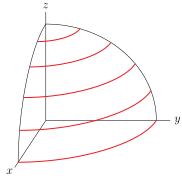
\includegraphics{sphericalLat.pdf}
\end{center}
\end{efig}
On the other hand, if you hold $\theta$ fixed and increase $\varphi$ 
by a small amount $\dee{\varphi}$, $\vr(\theta,\varphi)$ sweeps out the red circular 
arc in the figure on the left below. If you hold $\theta$ fixed  and vary 
$\varphi$ from $0$ to $\pi$, $\vr(\theta,\varphi)$ sweeps out a line of longitude.
The figure on the right below gives the lines of longitude
(or at least the parts of those lines in the first octant) for 
$\theta=0$, $\frac{\pi}{10}$, $\frac{2\pi}{10}$, $\frac{3\pi}{10}$, 
$\frac{4\pi}{10}$ and $\frac{5\pi}{10}=\frac{\pi}{2}$.
\begin{efig}
\begin{center}
    \includegraphics[scale=1.05]{sphericalPhi.pdf}\qquad
    \includegraphics{sphericalLong.pdf}
\end{center}
\end{efig}
\end{eg}

\begin{eg}[Cylinder]\label{SURclyinder}
The surface $x^2+z^2=1$ is an infinite cylinder. Part of this cylinder
in the first octant is sketched below.
\begin{nfig}
\begin{center}
    \includegraphics{cylinder.pdf}
\end{center}
\end{nfig}
Note that the section of this cylinder that lies in the $xz$-plane,
and in fact in any plane $y=c$, is the circle $x^2+z^2=1$. We can
of course parametrize this circle by $x=\cos\theta$, $z=\sin\theta$.
So we can parametrize the whole cylinder by using $\theta$ and $y$ 
as parameters.
\begin{equation*}
\vr(\theta,y) = \big(\cos\theta\,,\,y\,,\,\sin\theta\big)
\qquad
0\le\theta<2\pi,\ \ -\infty<y<\infty
\end{equation*}

\end{eg}

\begin{eg}[Surface of Revolution]\label{SURrevolution}
In this example, we are going to parametrize a surface of revolution.
In your first integral calculus course, you undoubtedly encountered
many surfaces created by rotating a curve $y=f(x)$ about the $x$-axis
or the $y$-axis. 
In this course, we are used to having the $z$-axis, rather than the $y$-axis, 
run vertically. 
%, and having the $y$-axis, rather than the $x$-axis, 
%run to the right. 
So in this example, we'll parametrize the surface 
constructed by rotating the curve 
\begin{equation*}
z=g(y)=e^y \qquad 0\le y\le 1
\end{equation*}
about the $z$-axis. Exactly the same procedure can be used to parametrize
surfaces created by rotating about the $x$-axis or the $y$-axis too.

We start by just sketching the curve, considering the $yz$-plane as 
the plane $x=0$ in $\bbbr^3$. The specified curve is the red curve 
in the figure below.
Concentrate on any one point on that curve. It is the blue dot at $(0,Y,e^Y)$
\vadjust{
\begin{nfig}
\begin{center}
    \includegraphics{revA.pdf}
\end{center}
\end{nfig}
}
in the figure. When our curve is rotated about the $z$-axis, the blue dot
sweeps out a circle. The circle that the blue dot sweeps out
\begin{itemize}\itemsep1pt \parskip0pt \parsep0pt %\itemindent-15pt
\item[$\circ$]
lies in the horizontal plane $z=e^Y$ and
\item[$\circ$]
is centred on the $z$-axis and
\item[$\circ$]
has radius $Y$.
\end{itemize}
We can parametrize the circle swept out in the usual way. Here
is a top view of the circle, with the parameter, named $\theta$, indicated. 
\begin{nfig}
\begin{center}
    \includegraphics{revTop.pdf}
\end{center}
\end{nfig}
The coordinates of the red dot are $\big(Y\sin\theta\,,\,Y\cos\theta\,,\,e^Y\big)$. This also gives 
a parametrization of the surface of revolution
\begin{align*}
x(Y,\theta) & = Y\sin\theta \\
y(Y,\theta) & = Y\cos\theta \\
z(Y,\theta) & = e^Y \\
&0\le Y\le 1,\qquad 0\le\theta<2\pi
\end{align*}
Notice, by way of checks, that
\begin{itemize}\itemsep1pt \parskip0pt \parsep0pt %\itemindent-15pt
\item[$\circ$] when $\theta=0$, 
\begin{equation*}
    \big(x(Y,0)\,,\,y(Y,0)\,,\,z(Y,0)\big)
                 =(0,Y,e^Y)
\end{equation*}
runs over the entire desired curve (namely $z=g(y)$, $0\le y\le 1$),  
when $Y$ runs over $0\le Y\le 1$ and
\item[$\circ$] for any fixed $0\le Y\le 1$, 
   $\big(x(Y,\theta)\,,\,y(Y,\theta)\,,\,z(Y,\theta)\big)$ runs over the circle
       $x^2+y^2=Y^2$, in the plane $z=e^Y$, 
       when $\theta$ runs over $0\le\theta<2\pi$.
\end{itemize}
Also notice that
\begin{equation*}
x(Y,\theta)^2 + y(Y,\theta)^2 = Y^2
\end{equation*}
so that
\begin{equation*}
Y=\sqrt{x(Y,\theta)^2 + y(Y,\theta)^2}
\end{equation*}
and
\begin{align*}
z(Y,\theta) =e^{Y} = e^{ \sqrt{x(Y,\theta)^2 + y(Y,\theta)^2} }
\end{align*}
That is, the surface of revolution is contained in the (infinite) surface
\begin{equation*}
z=e^{\sqrt{x^2+y^2}}
\end{equation*}
Remembering that $0\le Y\le 1$, we have that $1\le z=e^Y \le e$. 
Thus the surface of revolution is
\begin{equation*}
z=e^{\sqrt{x^2+y^2}}\qquad 1\le z\le e
\end{equation*}
Finally here is a sketch of the part of the surface in the first octant,
$x,y,z\ge 0$.
\begin{nfig}
\begin{center}
    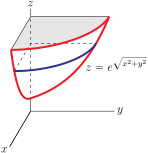
\includegraphics{revB.pdf}
\end{center}
\end{nfig}



\end{eg}

\begin{eg}[Torus]\label{SURdonut}
In this example, we are going to parametrize a donut (well, its surface), or an inner tube.
\begin{nfig}
\begin{center}
    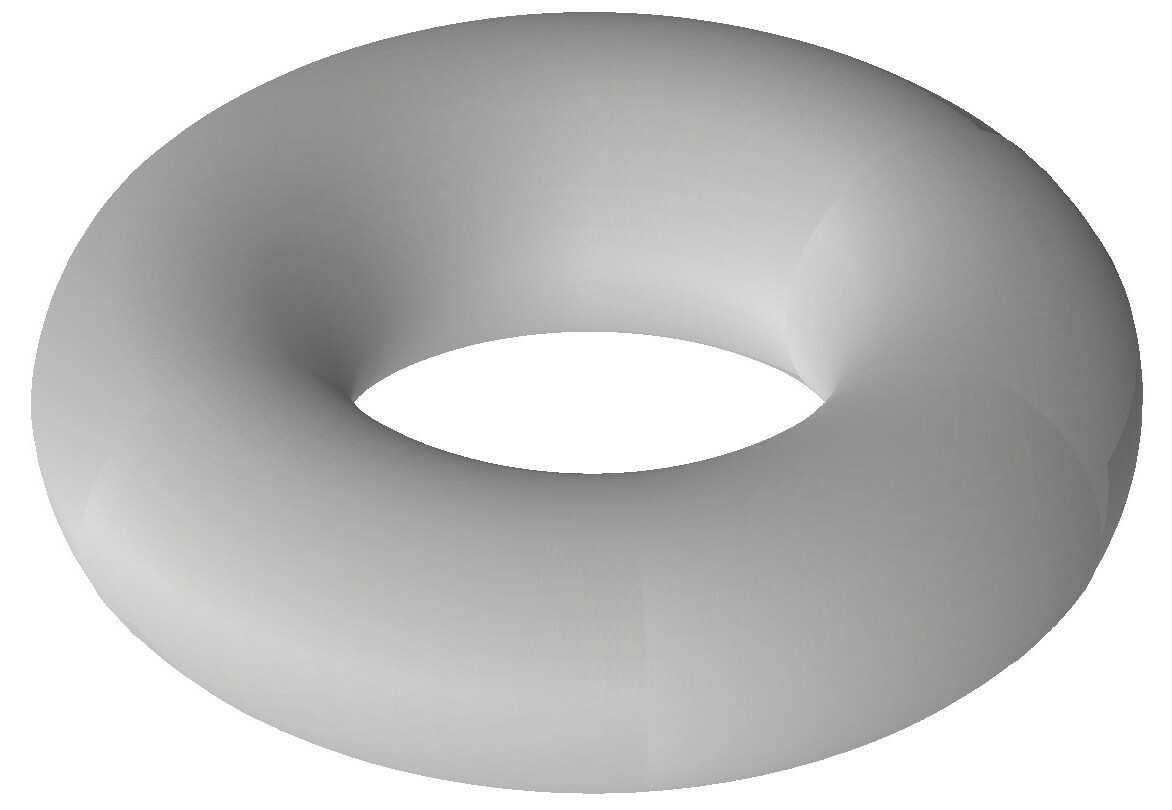
\includegraphics[scale=0.10]{torus3d.jpg}
\end{center}
\end{nfig}
The formal mathematical name for the surface of a donut is a torus. Our strategy will be to first parametrize the section of the torus in the 
right half of the
$yz$-plane,  and then built up the full torus by rotating the circle 
about the $z$-axis. The section is a circle, sketched below.
\vadjust{
\begin{nfig}
\begin{center}
    \includegraphics{torusSection.pdf}
\end{center}
\end{nfig}
}
We'll assume that the centre of the circle is a distance $R$ from the 
$z$-axis, and that the circle has radius $r$. Then the red dot on the circle 
is at
\begin{align*}
x&=0 \\
y&= R + r\cos\theta \\
z&= r\sin\theta
\end{align*}
In particular the red dot is a distance $r\sin\theta$ above the $xy$-plane and
is a distance $R + r\cos\theta$ from the $z$-axis. So when we rotate the section about the $z$-axis, the red dot sweeps out a circle
which is sketched below. 
\begin{efig}
\begin{center}
    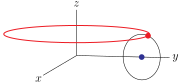
\includegraphics{torusRotB.pdf}
\end{center}
\end{efig}
The circle that the red dot sweeps out
\begin{itemize}\itemsep1pt \parskip0pt \parsep0pt %\itemindent-15pt
\item[$\circ$]
lies in the plane $z=r\sin\theta$ and
\item[$\circ$]
is centred on the $z$-axis and
\item[$\circ$]
has radius $\rho=R + r\cos\theta$.
\end{itemize}
We can parametrize the circle swept out in the usual way. Here
is a top view of the circle, with the parameter, named $\psi$, indicated. 
\begin{efig}
\begin{center}
    \includegraphics{torusTop.pdf}
\end{center}
\end{efig}
So the parametrization of the circle swept out by the red dot, and also the
parametrization of the torus, is
\begin{align*}
x &= \rho\cos\psi =  (R + r\cos\theta)\cos\psi \\
y &= \rho\sin\psi =  (R + r\cos\theta)\sin\psi \\
z &= r\sin\theta 
\end{align*}
or
\begin{equation*}
\vr(\theta,\psi) = (R + r\cos\theta)\cos\psi \ \hi
                    + (R + r\cos\theta)\sin\psi \ \hj
                    + r\sin\theta\ \hk
\qquad 0\le\theta,\psi < 2\pi
\end{equation*}


\end{eg}


\section{Tangent Planes}\label{sec:tangentPlanes}
If you are confronted with a complicated surface and want to get some
idea of what it looks like near a specific point, probably the first 
thing that you will do is find the plane that best approximates the 
surface near the point. That is, find the tangent plane to the surface at
the point. 
In general, a good way to specify a plane is to supply
\begin{itemize}\itemsep1pt \parskip0pt \parsep0pt %\itemindent-15pt
\item[$\circ$] 
a nonzero vector $\vn$ (called a normal vector) perpendicular to the 
plane\footnote{Alternatively, you could find two vectors that are in the 
plane (and not parallel to each other), and then construct a normal vector 
by taking their cross product.} (to determine the orientation of the plane) 
and
\item[$\circ$]
one point $(x_0,y_0,z_0)$ on the plane.
\end{itemize}
If $(x,y,z)$ is any other point on the plane, then the vector
\begin{equation*}
(x,y,z)-(x_0,y_0,z_0) = (x-x_0\,,\,y-y_0\,,\,z-z_0)
\end{equation*}
lies entirely in the plane and so is perpendicular to $\vn$. This gives 
the following very neat the equation for the plane.
\begin{equation*}
\vn\cdot(x-x_0\,,\,y-y_0\,,\,z-z_0) = 0\qquad
\raisebox{-30pt}[20pt][25pt]{\smash{\includegraphics{plane.pdf}}}
\end{equation*}
The following theorem provides formulae for normal vectors $\vn$ to 
general surfaces, assuming first that the surface is parametrized, 
second that the surface is a graph and finally the surface is given 
by an implicit equation. The formulae are developed in the proof of the
theorem.

\begin{theorem}[Normal vectors to surfaces]\label{thm:normalVectors}

\begin{enumerate}[(a)]

\item
Let
\begin{align*}
\vr&: \cD\subset\bbbr^2 \rightarrow \bbbr^3 \\
   &(u,v) \in\cD \mapsto \vr(u,v) =\big(x(u,v)\,,\,y(u,v)\,,\,z(u,v)\big)
\end{align*}
be a parametrized surface and let $(x_0,y_0,z_0)=\vr(u_0,v_0)$ 
be a point on the surface. Set
\begin{align*}
\vT_u &= \frac{\partial\ }{\partial u}\vr(u,v_0)\Big|_{u=u_0}
=\Big(\frac{\partial x}{\partial u}(u_0,v_0)\,,\,
      \frac{\partial y}{\partial u}(u_0,v_0)\,,\,
      \frac{\partial z}{\partial u}(u_0,v_0)\Big) \\
\vT_v &= \frac{\partial\ }{\partial v}\vr(u_0,v)\Big|_{v=v_0}
=\Big(\frac{\partial x}{\partial v}(u_0,v_0)\,,\,
      \frac{\partial y}{\partial v}(u_0,v_0)\,,\,
      \frac{\partial z}{\partial v}(u_0,v_0)\Big)
\end{align*}
Then
\begin{align*}
\vn = \vT_u\times\vT_v
=\det\left|\begin{matrix}
            \hi &  \hj & \hk \\[0.05in]
            \frac{\partial x}{\partial u}(u_0,v_0) &
                     \frac{\partial y}{\partial u}(u_0,v_0) &
                     \frac{\partial z}{\partial u}(u_0,v_0) \\[0.1in]
           \frac{\partial x}{\partial v}(u_0,v_0) &
                     \frac{\partial y}{\partial v}(u_0,v_0) &
                     \frac{\partial z}{\partial v}(u_0,v_0)
           \end{matrix}\right|
\end{align*}
is normal (i.e. perpendicular) to the surface at $(x_0,y_0,z_0)$.


\item
Let $(x_0,y_0,z_0)=f(x_0,y_0)$ be a point on the 
the surface $z=f(x,y)$. Then, 
\begin{align*}
\vn =-f_x(x_0,y_0)\,\hi - f_y(x_0,y_0)\,\hj + \hk
\end{align*}
is normal to the surface at $(x_0,y_0,z_0)$.

\item 
Consider the surface given implicitly by the equation $G(x,y,z) = K$, 
where $K$ is a constant. Let $(x_0,y_0,z_0)$ be a point on the surface and assume that the gradient $\vnabla G\big(x_0,y_0,z_0\big)\ne \vZero$. Then
\begin{align*}
\vn= \vnabla G\big(x_0,y_0,z_0\big)
\end{align*}
is normal to the surface at $(x_0,y_0,z_0)$.

\end{enumerate}

Note that none of the normal vectors $\vn$ above need be of unit length.
\end{theorem}
Note that if we apply part (c) to $G(x,y,z) = z - f(x,y)$ we get
the normal vector $\vn=\vnabla G\big(x_0,y_0,z_0\big)
   =-f_x(x_0,y_0)\,\hi - f_y(x_0,y_0)\,\hj + \hk$, which is the same as the
normal vector provided by part (b). Of course they had to be at least 
parallel.

\begin{proof} (a)
First fix $v=v_0$ and let $u$ vary. Then
\begin{equation*}
u\mapsto \vr(u,v_0) = \big(x(u,v_0)\,,\,y(u,v_0)\,,\,z(u,v_0)\big)
\end{equation*}
is a curve on the surface (the red curve in the figure on the right below) that
passes through $(x_0,y_0,z_0)$ (the black dot in the figure) when $u=u_0$.
\vadjust{
\begin{efig}
\begin{center}
    \null\hskip-0.1in
    \includegraphics[scale=0.95]{surfaceSlice.pdf}\quad 
    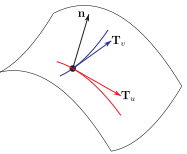
\includegraphics[scale=0.95]{saddleA.pdf}
    \hskip-0.1in\null
\end{center}
\end{efig}
}
The tangent vector to this curve at  $(x_0,y_0,z_0)$,
which is also a tangent vector to the surface at $(x_0,y_0,z_0)$,
is
\begin{equation*}
\vT_u = \frac{\partial\ }{\partial u}\vr(u,v_0)\Big|_{u=u_0}
=\Big(\frac{\partial x}{\partial u}(u_0,v_0)\,,\,
      \frac{\partial y}{\partial u}(u_0,v_0)\,,\,
      \frac{\partial z}{\partial u}(u_0,v_0)\Big)
\end{equation*}
It is the red arrow in the figure on the right above.

Next fix $u=u_0$ and let $v$ vary. Then
\begin{equation*}
v\mapsto \vr(u_0,v) = \big(x(u_0,v)\,,\,y(u_0,v)\,,\,z(u_0,v)\big)
\end{equation*}
is a curve on the surface (the blue curve in the figure on the right above) 
that passes through $(x_0,y_0,z_0)$ when $v=v_0$.
The tangent vector to this curve at  $(x_0,y_0,z_0)$,
which is also a tangent vector to the surface at $(x_0,y_0,z_0)$,
is
\begin{equation*}
\vT_v = \frac{\partial\ }{\partial v}\vr(u_0,v)\Big|_{v=v_0}
=\Big(\frac{\partial x}{\partial v}(u_0,v_0)\,,\,
      \frac{\partial y}{\partial v}(u_0,v_0)\,,\,
      \frac{\partial z}{\partial v}(u_0,v_0)\Big)
\end{equation*}
It is the blue arrow in the figure on the right above.

We now have two vectors, namely $\vT_u$ and $\vT_v$, that are tangent
to the surface at $(x_0,y_0,z_0)$. So their cross product
\begin{align*}
\vn = \vT_u\times\vT_v
=\det\left|\begin{matrix}
            \hi &  \hj & \hk \\[0.05in]
            \frac{\partial x}{\partial u}(u_0,v_0) &
                     \frac{\partial y}{\partial u}(u_0,v_0) &
                     \frac{\partial z}{\partial u}(u_0,v_0) \\[0.1in]
           \frac{\partial x}{\partial v}(u_0,v_0) &
                     \frac{\partial y}{\partial v}(u_0,v_0) &
                     \frac{\partial z}{\partial v}(u_0,v_0)
           \end{matrix}\right|
\end{align*}
is normal (i.e. perpendicular) to the surface at $(x_0,y_0,z_0)$.
Note however that this vector need not be normalized. That is, it need not 
be of unit length.

\bigskip
\noindent (b)
Next assume that the surface is given by the equation
$z=f(x,y)$. Then, renaming $u$ to $x$ and $v$ to $y$, we may reuse part (a):
\begin{equation*}
\vr(x,y) = \big(x,y, f(x,y)\big)
\end{equation*}
parametrizes the surface and, at $\big(x_0,y_0,z_0\big)=f(x_0,y_0)\big)$,
\begin{align*}
\vT_x &= \frac{\partial\vr }{\partial x}(x_0,y_0)
=\big(1\,,\,
      0\,,\,
      f_x(x_0,y_0)\big)
\\[0.05in]
\vT_y &= \frac{\partial\vr }{\partial y}(x_0,y_0)
=\big(0\,,\,
      1\,,\,
      f_y(x_0,y_0)\big)
\end{align*}
and
\begin{align*}
\vn &= \vT_x\times\vT_y
=\det\left|\begin{matrix}
            \hi &  \hj & \hk \\[0.05in]
            1 & 0 & f_x(x_0,y_0) \\[0.05in]
            0 & 1 & f_y(x_0,y_0)
           \end{matrix}\right|
=-f_x(x_0,y_0)\,\hi - f_y(x_0,y_0)\,\hj + \hk
\end{align*}

\bigskip
\noindent (c)
Finally assume that the surface is given implicitly by the equation
$G(x,y,z)=0$ or, more generally by the equation, $G(x,y,z) = K$, where $K$ is 
a constant. If $\vr(t)=\big(x(t)\,\,y(t)\,,\,z(t)\big)$ is any curve 
with $\vr(0) = (x_0,y_0,z_0)$ that lies on the surface, then 
\begin{alignat*}{5}
& & G\big(\vr(t)\big)&=K &\qquad &\text{for all $t$} \\
&\implies & \diff{\ }{t} G\big(x(t),y(t),z(t)\big)&=0 & &\text{for all $t$} 
\end{alignat*}
Applying the chain rule gives
\begin{align*}
\frac{\partial G}{\partial x}\big(x(t),y(t),z(t)\big)\diff{x}{t}(t)
+\frac{\partial G}{\partial y}\big(x(t),y(t),z(t)\big)\diff{y}{t}(t)
+\frac{\partial G}{\partial z}\big(x(t),y(t),z(t)\big)\diff{z}{t}(t)
&=0 
\end{align*}
The left hand side is exactly the dot product
of $\big(\frac{\partial G}{\partial x}
\,,\,\frac{\partial G}{\partial y}
\,,\,\frac{\partial G}{\partial z}\big)=\vnabla G$ 
with
$\big(\diff{x}{t}
\,,\,\diff{y}{t}
\,,\,\diff{z}{t}\big)
=\diff{\vr}{t}$, so that
\begin{align*}
\vnabla G\big(\vr(t)\big)\cdot\vr'(t)&=0 \qquad
          \text{for all $t$} \\
\implies  \vnabla G\big(x_0,y_0,z_0\big)\cdot\vr'(0)&=0 & 
\end{align*}
This tell us that $\vnabla G\big(x_0,y_0,z_0\big)$ is perpendicular
to $\vr'(0)$, which is a tangent vector to $G=K$ at $(x_0,y_0,z_0)$.
This is true for all curves $\vr(t)$ on $G=K$ and so is true
for all tangent vectors to $G=K$ at $(x_0,y_0,z_0)$.
So $\vnabla G\big(x_0,y_0,z_0\big)$ is a normal vector to $G(x,y,z)=K$ 
at $(x_0,y_0,z_0)$.

\end{proof} 

\begin{eg}\label{eg:tangentPlaneA}
Consider the surface
\begin{align*}
x &= x(u,v) = u\cos v \\
y &=y(u,v) = u\sin v \\
z &=z(u,v) = u 
\end{align*}
Observe that
\begin{equation*}
x(u,v)^2 + y(u,v)^2 = u^2 = z(u,v)^2
\end{equation*}
So our surface is also
\begin{equation*}
G(x,y,z) = x^2+y^2-z^2 = 0
\end{equation*}
We shall sketch it shortly. But first, let's find it's tangent plane
at $(x_0,y_0,z_0)=\vr(u_0,v_0)$.
In fact, let's do it twice. Once using the parametrization and once using its
implicit equation. First, using the parametrization 
$\vr(u,v) = u\cos v\,\hi + u\sin v\,\hj + u\,\hk$, we have
\begin{align*}
\vT_u &= \frac{\partial\vr}{\partial u}(u_0,v_0)
       =  \cos v_0\,\hi + \sin v_0\,\hj + \hk \\
\vT_v &= \frac{\partial\vr}{\partial v}(u_0,v_0)
       =  -u_0\sin v_0\,\hi + u_0\cos v_0\,\hj 
\end{align*}
so that
\begin{align*}
\vn &= \big(\cos v_0\,\hi + \sin v_0\,\hj + \hk\big)\times 
      \big(-u_0\sin v_0\,\hi + u_0\cos v_0\,\hj\big)\\
    &= \big(-u_0\cos v_0\,,\,-u_0\sin v_0\,,\, u_0)
      = (-x_0,-y_0,z_0)
\end{align*}
Next using the implicit equation $G(x,y,z) = x^2+y^2-z^2=0$, we have
the normal vector
\begin{equation*}
\vnabla G\big(x_0,y_0,z_0\big) = (2x_0,2y_0,-2z_0) =-2(-x_0,-y_0,z_0)
\end{equation*}
Of course the two vectors $(-x_0,-y_0,z_0)$ and $-2(-x_0,-y_0,z_0)$
are parallel to each other. Either can be used as a normal vector and
the tangent plane to $x^2+y^2-z^2=0$ at $(x_0,y_0,z_0)$ is
\begin{equation*}
0=\vn\cdot(x-x_0,y-y_0,z-z_0)
 = -x_0(x-x_0)-y_0(y-y_0) + z_0(z-z_0)
\end{equation*}
\emph{provided} $(x_0,y_0,z_0)\ne \vZero$. In the event that 
$(x_0,y_0,z_0) = \vZero$ the ``tangent plane equation'' reduces to $0=0$
and there is clearly a problem. 

More generally, if
$\vT_u\times\vT_v=\vZero$ (or $\vnabla G(x_0,y_0,z_0)=\vZero$), then
either\footnote{We saw the same dichotomy when considering what happened
for a curve when $\vr'(t)=0$. See Example \ref{eg:zeroSpeed}.}
\begin{itemize}
\item[$\circ$]
the surface fails to have a tangent plane at $(x_0,y_0,z_0)$, or
\item[$\circ$]
our parametrization is screwy\footnote{Of course ``screwy'' is not 
a mathematically precise word. One way a parametrization
$\vr(u,v)$ could be ``screwy'' is if it failed to give a 
one-to-one correspondence between parameter values $(u,v)$ and points
on (part of) the surface. For example, polar coordinates 
$\vr(u,v) = u\cos v\,\hi + u\sin v\,\hj$ give $\vr(0,v)=(0,0)$ for all
values of $v$.} there. For example, we can parametrize the 
$xy$-plane, $z=0$, by $\vr(u,v) = u\cos v\,\hi + u\sin v\,\hj$. (This is just
polar coordinates.) Then 
$\vT_u =  \cos v_0\,\hi + \sin v_0\,\hj $ and
$\vT_v =  -u_0\sin v_0\,\hi + u_0\cos v_0\,\hj$, so that
$\vT_u\times\vT_v = u_0\hk$ is $\vZero$ when $u_0=0$. But the plane $z=0$
is its own tangent plane everywhere. 
\end{itemize}
The surface of current interest is $x^2+y^2=z^2$. The intersection of 
this surface with the horizontal plane $z=z_0$ is $x^2+y^2=z_0^2$, which is
the circle of radius $|z_0|$ centred on $x=y=0$. So our surface is a stack of
circles. The radius of the circle in the $xy$-plane is zero. The radius
increases linearly as we move away from the $xy$-plane. Our surface
is a cone. It does not have a tangent plane at $(0,0,0)$. 
\begin{efig}
\begin{center}
    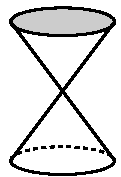
\includegraphics{cone.pdf}
\end{center}
\end{efig}

\end{eg}


\begin{eg}\label{eg:tangentPlaneB}
This time we shall find the tangent planes to the surface
\begin{equation*}
x^2 + y^2 -z^2 = 1
\end{equation*}
As for the cone of the last example, the intersection of 
this surface with the horizontal plane $z=z_0$ is a circle ---
the circle of radius $\sqrt{1+z_0^2}$  centred on $x=y=0$.
Our surface is again a stack of circles. The radius of the circle 
in the $xy$-plane is $1$. The radius increases as we move away from the $xy$-plane. Here is a sketch of the surface.
\begin{efig}
\begin{center}
    \includegraphics{hyperboloid1.pdf}
\end{center}
\end{efig}
It is called a hyperboloid\footnote{There are also hyperboloids of two sheets.
See Appendix \ref{ap:quadric}.} of one sheet. 

Using the implicit equation $G(x,y,z) = x^2+y^2-z^2=1$, we have
\begin{equation*}
\vnabla G\big(x_0,y_0,z_0\big) = (2x_0,2y_0,-2z_0) =2(x_0,y_0,-z_0)
\end{equation*}
and we may take $(x_0,y_0,-z_0)$ as a normal vector at $(x_0,y_0,z_0)$.
So the tangent plane to $x^2+y^2-z^2=1$ at $(x_0,y_0,z_0)$ is
\begin{equation*}
0=\vn\cdot(x-x_0,y-y_0,z-z_0)
 = x_0(x-x_0)+y_0(y-y_0) - z_0(z-z_0)
\end{equation*}
This time $\vn=(x_0,y_0,-z_0)\ne \vZero$, so that we have a tangent plane, at 
every point of the surface. In particular, the vanishing of 
$\vn=(x_0,y_0,-z_0)$ at $(x_0,y_0,z_0)=(0,0,0)$ is not a problem because 
$(0,0,0)$ is not on the surface.

\end{eg}

\begin{eg}[Optional --- Parametrizing the Hyperboloid of One Sheet]\label{eg:tangentPlaneBB}

The hyperboloid of one sheet, $x^2+y^2-z^2=1$, has a symmetry. It is 
invariant under rotation about the $z$-axis.
So it is natural to parametrize the surface using cylindrical coordinates.
\bigskip
\begin{align*}
x &= r\cos\theta \\
y &= r\sin\theta \\
z &= z \qquad\qquad
\qquad\raisebox{-20pt}[0pt][15pt]{\smash{\includegraphics{cylindrical.pdf}}}
\end{align*}
In cylindrical coordinates the surface $x^2+y^2-z^2=1$ is $r^2-z^2=1$,
and we could parametrize it by 
  $\vr(\theta,z) = \sqrt{1+z^2}\,\cos\theta\,\hi +\sqrt{1+z^2}\,\sin\theta\,\hj
      +z\,\hk$. Alternatively, we can eliminate the square roots in the
parametrization by exploiting the hyperbolic trig functions
\begin{equation*}
\sinh u = \frac{1}{2}\big(e^u-e^{-u}\big) \qquad
\cosh u = \frac{1}{2}\big(e^u+e^{-u}\big) \qquad
\end{equation*}  
The functions have properties\footnote{This is no accident: 
$\cosh u = \cos(iu)$ and $\sinh u = -i\sin(iu)$, where $i$ is the usual 
complex number that obeys $i^2=-1$. You can verify these formulae by just checking that $\cosh u$ and $\cos(iu)$ have the same Taylor expansions 
and that $\sinh u$ and $-i\sin(iu)$ have the same Taylor expansions.} 
that are very similar to those of $\sin\theta$ and $\cos\theta$.
\begin{align*}
\diff{\ }{u} \cosh u= \sinh u \qquad 
\diff{\ }{u} \sinh u= \cosh u \qquad 
\cosh^2 u -\sinh^2 u =1
\end{align*}
Observe that we can turn $r^2-z^2=1$ into $\cosh^2 u -\sinh^2 u =1$ simply by setting $r=\cosh u$, $z=\sinh u$. Doing so yields the parametrization
\begin{align*}
\vr(\theta,u) = \cosh u\,\cos\theta\,\hi +\cosh u\,\sin\theta\,\hj
      +\sinh u\,\hk
\end{align*}
As an exercise in working with hyperbolic trig functions, we'll use this
parametrization to find $\hn$. 
\begin{align*}
x&=  \cosh u\,\cos\theta &
x_u&=  \sinh u\,\cos\theta &
x_\theta&=  -\cosh u\,\sin\theta \\
%
y&= \cosh u\,\sin\theta &
y_u&= \sinh u\,\sin\theta &
y_\theta&= \phantom{-}\cosh u\,\cos\theta \\
%
z&=\sinh u &
z_u&=\cosh u &
z_\theta&=0
\end{align*}
So
\begin{align*}
\vn = \vT_u\times\vT_\theta
&=\det\left|\begin{matrix}
            \hi &  \hj & \hk \\
            \sinh u\,\cos\theta &
               \sinh u\,\sin\theta &
               \cosh u \\[0.1in]
           -\cosh u\,\sin\theta  &
            \cosh u\,\cos\theta &
             0
           \end{matrix}\right| \\
&=\big(-\cosh^2u\,\cos\theta\,,\,
       -\cosh^2u\,\sin\theta\,,\,
       \sinh u\cosh u\big)
\end{align*}
\end{eg}


\section{Surface Integrals}\label{sec:surfaceIntegrals}

We are now going to define two types of integrals over surfaces.
\begin{itemize}
\item[$\circ$]
  Integrals that look like $\dblInt_S \rho\,\dee{S}$ are used to
compute the area and, when $\rho$ is, for example, a mass density,
the mass of the surface $S$.
\item[$\circ$]
  Integrals that look like $\dblInt_S \vF\cdot\hn\,\dee{S}$,
with $\hn(x,y,z)$ being a unit vector that is perpendicular to 
$S$ at $(x,y,z)$,  are called
flux integrals. We shall see in \S\ref{sec:fluxIntegrals}, that when
$\vv$ is the velocity field of a moving fluid and $\rho$ is the density
of the fluid, then $\dblInt_S \rho\vv\cdot\hn\,\dee{S}$ is the rate at which
fluid is crossing the surface $S$.
\end{itemize}

\subsection{Parametrized Surfaces}\label{subsec:paramSurfaces}
Suppose that we wish to integrate over part, $S$, of a surface that is
parametrized by $\vr(u,v)$. We start by cutting $S$ up into small pieces
by drawing a bunch of curves of constant $u$ (the blue curves in the
figure below) and a bunch of curves of constant $v$ (the red curves in the
figure below).
\begin{nfig}
\begin{center}
    \includegraphics[scale=0.7]{surfaceSlice.pdf}
\end{center}
\end{nfig}
Concentrate on any one the small pieces. Here is a greatly magnified
sketch.
\begin{nfig}
\begin{center}
    \includegraphics{dS.pdf}
\end{center}
\end{nfig}
For example, the  lower red curve was constructed by holding $v$ fixed 
at the value $v_0$, varying $u$ and sketching $\vr(u,v_0)$, and 
the  upper red curve was constructed by holding $v$ fixed 
at the slightly larger value $v_0+\dee{v}$, varying $u$ and 
sketching $\vr(u,v_0+\dee{v})$. So the four intersection points in 
the figure are
\begin{alignat*}{3}
P_2&=\vr(u_0, v_0+\dee{v}) &\qquad
   P_3&=\vr(u_0+\dee{u}, v_0+\dee{v}) \\
P_0&=\vr(u_0, v_0) &
   P_1&=\vr(u_0+\dee{u}, v_0) 
\end{alignat*}
Now if
\begin{equation*}
\vR(t) = \vr(u_0+t\dee{U}\,,\,v_0+t\dee{V})
\end{equation*}
(where $\dee{U}$ and $\dee{V}$ are any small constants)
then, by Taylor expansion,
\begin{align*}
\vr\big(u_0+\dee{U}\,,\,v_0+\dee{V}\big)
&=\vR(1) \\
&\approx \big[\vR(0) +\vR'(0)\,\big(t-0\big)\big]_{t=1} \\
&=\vr(u_0\,,\,v_0)
   +\frac{\partial\vr}{\partial u}(u_0\,,\,v_0)\,\dee{U}
   +\frac{\partial\vr}{\partial v}(u_0\,,\,v_0)\,\dee{V}
\end{align*}
Applying this three times, once with $\dee{U}=\dee{u}$, $\dee{V}=0$,
once with $\dee{U}=0$ $\dee{V}=\dee{v}$, and once with 
$\dee{U}=\dee{u}$, $\dee{V}=\dee{v}$,
\begin{alignat*}{3}
P_0&=\vr(u_0\,,\,v_0) \\
P_1&=\vr(u_0+\dee{u}, v_0)
   &&\approx \vr(u_0\,,\,v_0)
   +\frac{\partial\vr}{\partial u}(u_0\,,\,v_0)\,\dee{u} \\
P_2&=\vr(u_0, v_0+\dee{v})
   &&\approx \vr(u_0\,,\,v_0)
   +\frac{\partial\vr}{\partial v}(u_0\,,\,v_0)\,\dee{v} \\
P_3&=\vr(u_0+\dee{u}, v_0+\dee{v})
   &&\approx\vr(u_0\,,\,v_0)
   +\frac{\partial\vr}{\partial u}(u_0\,,\,v_0)\,\dee{u}
   +\frac{\partial\vr}{\partial v}(u_0\,,\,v_0)\,\dee{v} 
\end{alignat*}
We have dropped all Taylor expansion terms that are of degree two or higher 
in $\dee{u}$, $\dee{v}$. The reason is that, in defining the integral, we take 
the limit $\dee{u},\dee{v}\rightarrow 0$. Because of that limit, 
all of the dropped terms contribute exactly $0$ to the integral. 
We shall not prove this. But we shall show, in the optional
\S\ref{sec:hoterms}, why this is the case.  

The small piece of our
surface with corners $P_0$, $P_1$, $P_2$, $P_3$  is approximately a parallelogram with sides
\begin{align*}
\overrightarrow{P_0P_1}
\approx \overrightarrow{P_2P_3}
&\approx \frac{\partial\vr}{\partial u}(u_0\,,\,v_0)\,\dee{u}  \\
\overrightarrow{P_0P_2}
\approx \overrightarrow{P_1P_3}
&\approx \frac{\partial\vr}{\partial v}(u_0\,,\,v_0)\,\dee{v}  
\qquad\qquad
\raisebox{-15pt}[20pt][10pt]{\smash{\includegraphics{dS2.pdf}}}
\end{align*}
Denote by $\theta$ the angle between the vectors 
$\overrightarrow{P_0P_1}$ and $\overrightarrow{P_0P_2}$.
The base of the parallelogram, $\overrightarrow{P_0P_1}$,
has length $\big|\overrightarrow{P_0P_1}\big|$, and the height of the
parallelogram is $\big|\overrightarrow{P_0P_2}\big|\,\sin\theta$.
So the area of the parallelogram is\footnote{As we mentioned above,
the approximation below becomes exact when the limit $\dee{u},\dee{v}\rightarrow 0$ is taken in the definition of the integral.
See the optional \S\ref{sec:hoterms}.}
\begin{align*}
|\overrightarrow{P_0P_1}|\ |\overrightarrow{P_0P_2}| \ \sin\theta
&= \big|\overrightarrow{P_0P_1}\times\overrightarrow{P_0P_2}\big| \\
&\approx \bigg|\frac{\partial\vr}{\partial u}(u_0\,,\,v_0)\times
              \frac{\partial\vr}{\partial v}(u_0\,,\,v_0)\bigg|
          \dee{u}\dee{v}
\end{align*}
Furthermore, $\frac{\partial\vr}{\partial u}(u_0\,,\,v_0)$
and $\frac{\partial\vr}{\partial v}(u_0\,,\,v_0)$
are tangent vectors to the curves $\vr(t\,,\,v_0)$ and $\vr(u_0\,,\,t)$
respectively. Both of these curves lie in $S$.
So $\frac{\partial\vr}{\partial u}(u_0\,,\,v_0)$
and $\frac{\partial\vr}{\partial v}(u_0\,,\,v_0)$ are tangent
vectors to $S$ at $(u_0,v_0)$ and the cross product
$\frac{\partial\vr}{\partial u}(u_0\,,\,v_0)\times
              \frac{\partial\vr}{\partial v}(u_0\,,\,v_0)$
is perpendicular to $S$ at $(u_0,v_0)$. We have found
both $\dee{S}$ and $\hn\,\dee{S}$, where $\hn$ is a unit normal vector
to the surface.
\begin{impeqn}\label{eq:SUdSparam}
For the parametrized surface $\vr(u,v)$,
\begin{align*}
\hn\, \dee{S} & = \pm\frac{\partial\vr}{\partial u}(u\,,\,v)\times
              \frac{\partial\vr}{\partial v}(u\,,\,v)\ 
          \dee{u}\dee{v} \\[0.1in]
\dee{S}&= \bigg|\frac{\partial\vr}{\partial u}(u\,,\,v)\times
              \frac{\partial\vr}{\partial v}(u\,,\,v)\bigg|\ 
          \dee{u}\dee{v}
\end{align*}
\end{impeqn}

\noindent
The $\pm$ sign in \eqref{eq:SUdSparam} is there because there are
two unit normal vectors at each point of a surface, one on each side of the
surface. Typically, the application itself tells you 
which of the two normal vectors should be used. We shall see many examples shortly.

\subsection{Graphs}
The surface which is the graph $z = f(x,y)$ can be parametrized
by 
\begin{equation*}
\vr(x,y) = x\,\hi + y\,\hj + f(x,y)\,\hk
\end{equation*} 
As
\begin{align*}
\frac{\partial\vr}{\partial x}  
       = \hi + \frac{\partial f}{\partial x}\,\hk \qquad\text{and}\qquad
\frac{\partial\vr}{\partial y}  
       = \hj + \frac{\partial f}{\partial y}\,\hk 
\end{align*}
we have
\begin{equation*}
 \frac{\partial\vr}{\partial x}\times
              \frac{\partial\vr}{\partial y}
=\det\left[\begin{matrix}
           \hi & \hj & \hk \\
           1 & 0 & \frac{\partial f}{\partial x} \\[0.05in]
           0 & 1 & \frac{\partial f}{\partial y}
           \end{matrix}\right]
= -f_x(x,y)\,\hi - f_y(x,y)\,\hj + \hk
\end{equation*}
So, \eqref{eq:SUdSparam} gives the following.
\begin{impeqn}\label{eq:SUdSgraph}
For the surface $z=f(x,y)$,
\begin{align*}
\hn\, \dee{S} & = \pm\big[-f_x(x,y)\,\hi - f_y(x,y)\,\hj + \hk\big]\ 
          \dee{x}\dee{y} \\[0.1in]
\dee{S}&= \sqrt{1 + f_x(x,y)^2 + f_y(x,y)^2}\ 
          \dee{x}\dee{y}
\end{align*}
Similarly, for the surface $x=g(y,z)$, 
\begin{align*}
\hn\, \dee{S} & = \pm\big[\hi -g_y(y,z)\,\hj - g_z(y,z)\,\hk\big]\ 
          \dee{y}\dee{z} \\[0.1in]
\dee{S}&= \sqrt{1 + g_y(y,z)^2 + g_z(y,z)^2}\ 
          \dee{y}\dee{z}
\end{align*}
and for the surface $y=h(x,z)$,
\begin{align*}
\hn\, \dee{S} & = \pm\big[-h_x(x,z)\,\hi +\hj - h_z(x,z)\,\hk\big]\ 
          \dee{x}\dee{z} \\[0.1in]
\dee{S}&= \sqrt{1 + h_x(x,z)^2 + h_z(x,z)^2}\ 
          \dee{x}\dee{z}
\end{align*}
\end{impeqn}
\noindent
Again, in any given application, some care must be taken in choosing
the sign in \eqref{eq:SUdSgraph}, so as to get the appropriate 
normal vector.

The formulae like 
$\dee{S}= \sqrt{1 + f_x(x,y)^2 + f_y(x,y)^2}\ \dee{x}\dee{y}$
in \eqref{eq:SUdSgraph} have geometric interpretations. The red
parallelogram in the sketch
\begin{nfig}
\begin{center}
    \includegraphics{surfaceProj.pdf}
\end{center}
\end{nfig}
represents a little piece of our surface. It has area
$\dee{S}= \sqrt{1 + f_x(x,y)^2 + f_y(x,y)^2}\ \dee{x}\dee{y}$.
The blue parallelogram in the same sketch represents the projection
of the red parallelogram onto the $xy$-plane. It has area $\dee{x}\dee{y}$.
The vector $\hn$ in the sketch is a unit normal for the red parallelogram.
We have seen that it is parallel to 
\begin{equation*}
\frac{\partial\vr}{\partial x}\times
              \frac{\partial\vr}{\partial y}
= -f_x(x,y)\,\hi - f_y(x,y)\,\hj + \hk
\end{equation*}
so that the angle $\theta$ between $\hn$ and $\hk$ obeys
\begin{align*}
\cos\theta &= \frac{(-f_x(x,y)\,\hi - f_y(x,y)\,\hj + \hk)\cdot\hk}
                 {\big|-f_x(x,y)\,\hi - f_y(x,y)\,\hj + \hk\big|\,|\hk|} \\
&=\frac{1}{\sqrt{1 + f_x(x,y)^2 + f_y(x,y)^2}}
\end{align*}
The geometric interpretation of 
$\dee{S}= \sqrt{1 + f_x(x,y)^2 + f_y(x,y)^2}\ \dee{x}\dee{y}$
is that the area $\dee{S}$ of a little piece of surface is the
area of its projection on the $xy$-plane times the factor
$\frac{1}{\cos\theta}$ where $\theta$ is the angle between $\hn$
(which is perpendicular to the surface) and $\hk$ (which is
perpendicular to the $xy$-plane). Notice that
\begin{itemize}\itemsep1pt \parskip0pt \parsep0pt %\itemindent-15pt
\item[$\circ$]
when $\theta$ is close to zero, which corresponds the $f$ being almost constant
and our surface being almost parallel to the $xy$-plane, $\dee{S}$ 
reduces to almost $\dee{x}\dee{y}$.

\item[$\circ$]
On the other hand, in the limit $\theta\rightarrow\frac{\pi}{2}$, which 
corresponds to $f_x$ and/or $f_y$ becoming infinite
and our surface becoming perpendicular to the $xy$-plane, 
$\dee{S}$ becomes ``infinity times'' $\dee{x}\dee{y}$. In this case,
we should represent our surface either in the form $x=g(y,z)$ 
or in the form $y=h(x,z)$, rather than in the form $z=f(x,y)$.

\end{itemize}


\subsection{Surfaces Given by Implicit Equations}
Finally suppose that the surface is given by the equation
$G(x,y,z)=K$, with $K$ a constant. Suppose further that at some point 
on the surface $\frac{\partial G}{\partial z} \ne 0$. Then near that point 
we may solve\footnote{This is called the implicit function theorem. We 
will not prove it. But it is not so hard to understand why it is true, if one thinks in terms of the Taylor expansion of
$G$ about the point. For simplicity, let's suppose that the point is
$(0,0,0)$ and $G$ happens to be exactly equal to its first order 
Taylor expansion about $(0,0,0)$. That is, $G(x,y,z) = A +Bx +Cy +Dz$,
for some constants $A$, $B$, $C$, $D$. Since $(0,0,0)$ is on the surface,
$A=K$. As $\frac{\partial G}{\partial z}=D \ne 0$  we can easily solve
$G(x,y,z)=K$ for $z$ as a function of $x$ and $y$. Namely
$z=\frac{1}{D}(-Bx-Cy)$. The general proof is based on the fact that,
under reasonable hypotheses, the first order Taylor expansion is a 
good approximation to $G$ near $(0,0,0)$.} 
the equation $G(x,y,z)=K$ for $z$ as a function of $x$ and $y$. That is, the surface also obeys $z=f(x,y)$ for a function $f(x,y)$
that satisfies 
\begin{equation*}
G\big(x,y,f(x,y)\big) = K
\end{equation*}
near the point.
Differentiating this with respect to $x$ and $y$ gives, by the chain rule,
\begin{alignat*}{3}
0&=\frac{\partial\hfill}{\partial x}\Big[G\big(x,y,f(x,y)\big)\Big]
 &\ =\ G_x\big(x,y,f(x,y)\big) + G_z\big(x,y,f(x,y)\big)\,f_x(x,y) \\ 
0&=\frac{\partial\hfill}{\partial y}\Big[G\big(x,y,f(x,y)\big)\Big]
 &\ =\ G_y\big(x,y,f(x,y)\big) + G_z\big(x,y,f(x,y)\big)\,f_y(x,y)
\end{alignat*}
which implies
\begin{align*}
f_x(x,y) = -\frac{G_x\big(x,y,f(x,y)\big)}{G_z\big(x,y,f(x,y)\big)}
\qquad
f_y(x,y) = -\frac{G_y\big(x,y,f(x,y)\big)}{G_z\big(x,y,f(x,y)\big)}
\end{align*}
and
\begin{align*}
-f_x(x,y)\,\hi - f_y(x,y)\,\hj + \hk
&=\frac{G_x\big(x,y,f(x,y)\big)}{G_z\big(x,y,f(x,y)\big)}\,\hi+
\frac{G_y\big(x,y,f(x,y)\big)}{G_z\big(x,y,f(x,y)\big)}\,\hj+\hk \\
&=\frac{\vnabla G\big(x,y,f(x,y)\big)}{G_z\big(x,y,f(x,y)\big)}
\end{align*}
So, by (\ref{eq:SUdSgraph}),
\begin{impeqn}\label{eq:SUdSimplicit}
For the surface $G(x,y,z)=K$, when $G_z(x,y,z)\ne 0$,
\begin{align*}
\hn\, \dee{S} & = 
    \pm\frac{\vnabla G\big(x,y,z\big)}{\vnabla G\big(x,y,z\big)\cdot\hk}\ 
          \dee{x}\dee{y} \\[0.1in]
\dee{S}&= 
\bigg|\frac{\vnabla G\big(x,y,z\big)}{\vnabla G\big(x,y,z\big)\cdot\hk}\bigg|\ 
          \dee{x}\dee{y}
\end{align*}
Similarly, for the surface $G(x,y,z)=K$, when $G_x(x,y,z)\ne 0$,
\begin{align*}
\hn\, \dee{S} & = 
    \pm\frac{\vnabla G\big(x,y,z\big)}{\vnabla G\big(x,y,z\big)\cdot\hi}\ 
          \dee{y}\dee{z} \\[0.1in]
\dee{S}&= 
\bigg|\frac{\vnabla G\big(x,y,z\big)}{\vnabla G\big(x,y,z\big)\cdot\hi}\bigg|\ 
          \dee{y}\dee{z}
\end{align*}
and for the surface $G(x,y,z)=K$, when $G_y(x,y,z)\ne 0$,
\begin{align*}
\hn\, \dee{S} & = 
    \pm\frac{\vnabla G\big(x,y,z\big)}{\vnabla G\big(x,y,z\big)\cdot\hj}\ 
          \dee{x}\dee{z} \\[0.1in]
\dee{S}&= 
\bigg|\frac{\vnabla G\big(x,y,z\big)}{\vnabla G\big(x,y,z\big)\cdot\hj}\bigg|\ 
          \dee{x}\dee{z}
\end{align*}

\end{impeqn}
\noindent
If, for some point $(x_0,y_0,z_0)$ we have 
$G_x(x_0,y_0,z_0)= 
 G_y(x_0,y_0,z_0)= 
 G_z(x_0,y_0,z_0)= 0$, we also have a problem! Often this is a sign
that our surface is not smooth at $(x_0,y_0,z_0)$ and in fact does not
have a normal vector there. For an example of this, see 
Example \ref{eg:tangentPlaneA}.


\subsection{Examples of $\dblInt_S \rho\,\dee{S}$}\label{sec:rhodSexamples}
We'll start by computing, in several different ways, the surface area of the 
hemisphere
\begin{equation*}
x^2+y^2+z^2=a^2\qquad z\ge 0
\end{equation*}
(with $a>0$).
You probably know, from high school, that the answer is 
$\frac{1}{2}\times 4\pi a^2=2\pi a^2$. But you have probably 
not seen a derivation of this answer.
Note that, since $x^2+y^2 = a^2-z^2$ on the hemisphere, the set
of $(x,y)$'s for which there is a $z$ with $(x,y,z)$ on the  hemisphere
is exactly $\Set{(x,y)\in\bbbr^2}{x^2+y^2\le a^2}$.

\begin{eg}[Area of a hemisphere --- using cylindrical coordinates]
       \label{eg:SphereAreaCyl}
Let's parametrize the hemisphere $x^2+y^2+z^2=a^2$, $z\ge 0$, 
using as parameters the polar coordinates $r$, $\theta$ of the 
cylindrical coordinates\footnote{The symbols $r$, $\theta$, $z$
are the standard mathematics symbols for the cylindrical coordinates. Appendix \ref{ap:ISO} gives another set of symbols that is commonly used in the physical sciences and engineering.} 
\bigskip
\begin{align*}
x &= r\cos\theta \\
y &= r\sin\theta \\
z &= z \qquad\qquad
\qquad\raisebox{-20pt}[0pt][15pt]{\smash{\includegraphics{cylindrical.pdf}}}
\end{align*}
and then apply \eqref{eq:SUdSparam}.
In cylindrical coordinates the equation $x^2+y^2+z^2=a^2$
becomes $r^2+z^2=a^2$, and the condition $x^2+y^2\le a^2$ is $0\le r\le a$, 
$0\le\theta< 2\pi$. 

So the hemisphere can be parametrized by
\begin{align*}
%\vR(r,\theta) =
&\big(x(r,\theta)\,,\, y(r,\theta)\,,\, z(r,\theta)\big)
=\big(r\cos\theta\,,\,r\sin\theta\,,\,\sqrt{a^2-r^2}\,\big)\\
&\hskip1in\text{with }\ 
0\le r\le a,\ 0\le\theta<2\pi
\end{align*}
Note that we selected the positive solution $z=\sqrt{a^2-r^2}$ of $r^2+z^2=a^2$
in order to satisfy the condition that $z\ge 0$.
Since
\begin{align*}
\Big(\frac{\partial x}{\partial r}\,,\,\frac{\partial y}{\partial r}\,,\,
                     \frac{\partial z}{\partial r}\Big)
&=\Big(\cos\theta\,,\,\sin\theta\,,\,-\frac{r}{\sqrt{a^2-r^2}}\Big)\\
\Big(\frac{\partial x}{\partial\theta}\,,\,\frac{\partial y}{\partial\theta}
             \,,\, \frac{\partial z}{\partial\theta}\Big)
&=(-r\sin\theta\,,\,r\cos\theta\,,\,0) 
\end{align*}
\eqref{eq:SUdSparam} yields
\begin{align*}
\hn\,\dee{S}
&=\pm\Big(\frac{\partial x}{\partial r}\,,\,\frac{\partial y}{\partial r}
   \,,\,\frac{\partial z}{\partial r}\Big)
\times
\Big(\frac{\partial x}{\partial\theta}\,,\,\frac{\partial y}{\partial\theta}
   \,,\, \frac{\partial z}{\partial\theta}\Big)
\ \dee{r}\dee{\theta}\\
%&=\pm \Big(\cos\theta\,,\,\sin\theta\,,\,-\frac{r}{\sqrt{a^2-r^2}}\Big)
%\times
%(-r\sin\theta\,,\,r\cos\theta\,,\,0) 
%\ \dee{r}\dee{\theta}\\
&=\pm \det\left[\begin{matrix}
                \hi & \hj & \hk \\
                \cos\theta & \sin\theta & -\frac{r}{\sqrt{a^2-r^2}} \\
                -r\sin\theta & r\cos\theta & 0
                \end{matrix}\right]\ \dee{r}\dee{\theta}
\\
&=\pm\Big(\frac{r^2\cos\theta}{\sqrt{a^2-r^2}}\,,\,
           \frac{r^2\sin\theta}{\sqrt{a^2-r^2}}\,,\,
          r\Big)\ \dee{r}\dee{\theta} \\
\dee{S}&=\sqrt{ \frac{r^4}{a^2-r^2} +r^2}\ \dee{r}\dee{\theta}
        =\sqrt{ \frac{a^2r^2}{a^2-r^2}}\ \dee{r}\dee{\theta}
        =\frac{ar}{\sqrt{a^2-r^2}}\ \dee{r}\dee{\theta}
\end{align*}
So the area of the hemisphere is
\begin{align*}
\int_0^a \dee{r}\int_0^{2\pi}\dee{\theta}\ \frac{ar}{\sqrt{a^2-r^2}}
&=2\pi a\int_0^a \dee{r}\ \frac{r}{\sqrt{a^2-r^2}}
%=2\pi a\Big[-\sqrt{a^2-r^2}\Big]_0^a
%=2\pi a^2
\\
&=2\pi a\int_{a^2}^0 \frac{-\dee{u}/2}{\sqrt{u}}
\qquad\text{with $u=a^2-r^2,\ \dee{u} = -2r\,\dee{r}$} \\
&=2\pi a\Big[-\sqrt{u}\Big]_{a^2}^0 \\
&=2\pi a^2
\end{align*}
as it should be.
\end{eg}


\begin{eg}[Area of a hemisphere --- using an implicit equation]
       \label{eg:SphereImplicit}
This time we'll compute the area of the hemisphere by using that, if
$(x,y,z)$ is on the hemisphere, then $G(x,y,z) = a^2$ with 
$G(x,y,z) = x^2 + y^2 + z^2$.
Since 
\begin{equation*}
\vnabla G(x,y,z) = \big(2x\,,\,2y\,,\,2z\big)
\end{equation*}
\eqref{eq:SUdSimplicit} yields
\begin{align*}
\dee{S}
&= \bigg|\frac{\vnabla G\big(x,y,z\big)}{\vnabla G\big(x,y,z\big)\cdot\hk}\bigg|
            \ \dee{x}\dee{y} \\
&= \bigg|\frac{\big(2x\,,\,2y\,,\,2z\big)}{2z}\bigg|
            \ \dee{x}\dee{y} \\
&= \frac{\sqrt{x^2+y^2+z^2}}{|z|}
            \ \dee{x}\dee{y} \\
&= \frac{a}{\sqrt{a^2-x^2-y^2}}
            \ \dee{x}\dee{y} \qquad\text{on $x^2+y^2+z^2=a^2$}
\end{align*}
So the area is
$
\dblInt_{x^2+y^2\le a^2}\frac{a}{\sqrt{a^2-x^2-y^2}}
            \ \dee{x}\dee{y} 
$.
To evaluate this integral, we switch to polar coordinates, substituting
$x=r\cos\theta$, $y=r\sin\theta$. This gives
\begin{align*}
\text{area}
&=\dblInt_{x^2+y^2\le a^2}\frac{a}{\sqrt{a^2-x^2-y^2}}
            \ \dee{x}\dee{y} 
=\int_0^a\dee{r}\ r\int_0^{2\pi}\dee{\theta}\  \frac{a}{\sqrt{a^2-r^2}} \\
&=2\pi a \int_0^a\dee{r}\ \frac{r}{\sqrt{a^2-r^2}}
\end{align*}
We already showed, in Example \ref{eg:SphereAreaCyl}, that the value
of this integral is $2\pi a^2$.
\end{eg}


\begin{eg}[Area of a hemisphere --- using spherical coordinates]
       \label{eg:SphereAreaSC}
Of course ``integrating over a sphere'' cries out  for 
spherical coordinates. So
this time we parametrize the hemisphere $x^2+y^2+z^2=a^2$, $z\ge 0$, 
using as parameters the angular coordinates $\theta$, $\varphi$ of the 
spherical coordinates 
\vskip0.35in
\begin{align*}
x&=\rho\sin\varphi\cos\theta \\
y&=\rho\sin\varphi\sin\theta \\
z&=\rho\cos\varphi\qquad\qquad
\raisebox{-30pt}[0pt][15pt]{\smash{\includegraphics[scale=0.95]{spherical.pdf}}}
\end{align*}
\vskip0.4in
\noindent and then apply \eqref{eq:SUdSparam}.
In spherical coordinates the equation $x^2+y^2+z^2=a^2$
becomes just $\rho^2=a^2$, and the condition $z\ge 0$ is $0\le\varphi\le\frac{\pi}{2}$, $0\le\theta< 2\pi$. 
So the hemisphere can be parametrized\footnote{As we have noted before,
the spherical coordinate system really breaks down at $\varphi=0$,
because $\rho=1$, $\varphi=0$ gives the same point, namely the north pole $(0,0,1)$, for all values of $\theta$. We should really treat our
integral like an improper integral, first integrating over
$\veps<\varphi\le\frac{\pi}{2}$ and then taking the limit 
$\veps\rightarrow 0^+$.
However the breakdown of the spherical coordinate system at $\varphi=0$,
just like the breakdown of polar coordinates at $r=0$, rarely causes
problem and it is routine to skip the ``improper integral'' step.} by
\begin{equation*}
\big(x(\theta,\varphi)\,,\, y(\theta,\varphi)\,,\, z(\theta,\varphi)\big)
=\big(a\sin\varphi\cos\theta\,,\,a\sin\varphi\sin\theta\,,\,a\cos\varphi\,\big)\quad
0\le\varphi\le\frac{\pi}{2},\ 0\le\theta<2\pi
\end{equation*}
Since
\begin{align*}
\Big(\frac{\partial x}{\partial\theta}\,,\,
      \frac{\partial y}{\partial\theta}\,,\,
      \frac{\partial z}{\partial\theta}\Big)
&=\big(-a\sin\varphi\sin\theta\,,\,
       a\sin\varphi\cos\theta\,,\,0\big)\\
\Big(\frac{\partial x}{\partial\varphi}\,,\,\frac{\partial y}{\partial\varphi}
             \,,\, \frac{\partial z}{\partial\varphi}\Big)
&=(a\cos\varphi\cos\theta\,,\,a\cos\varphi\sin\theta\,,\,-a\sin\varphi) 
\end{align*}
\eqref{eq:SUdSparam} yields
\begin{align*}
\hn\,\dee{S}
&=\pm\Big(\frac{\partial x}{\partial\theta}\,,\,
          \frac{\partial y}{\partial\theta}\,,\,
          \frac{\partial z}{\partial\theta}\Big)
\times
\Big(\frac{\partial x}{\partial\varphi}\,,\,\frac{\partial y}{\partial\varphi}
   \,,\, \frac{\partial z}{\partial\varphi}\Big)
\ \dee{\theta}\dee{\varphi}\\
&=\pm \big(-a\sin\varphi\sin\theta\,,\,
       a\sin\varphi\cos\theta\,,\,0\big)
\times
(a\cos\varphi\cos\theta\,,\,a\cos\varphi\sin\theta\,,\,-a\sin\varphi)
\ \dee{\theta}\dee{\varphi}\\
&=\pm\big(-a^2\sin^2\varphi\cos\theta\,,\,
          -a^2\sin^2\varphi\sin\theta\,,\,
          -a^2\sin\varphi\cos\varphi\Big)\ \dee{\theta}\dee{\varphi} \\
&=\mp a^2\sin\varphi \big(\sin\varphi\cos\theta\,,\,
          \sin\varphi\sin\theta\,,\,
          \cos\varphi\Big)\ \dee{\theta}\dee{\varphi} \\
\dee{S}&=a^2\sin\varphi \sqrt{\sin^2\varphi\cos^2\theta
                    +\sin^2\varphi\sin^2\theta
                    +\cos^2\varphi}\ \dee{\theta}\dee{\varphi}\\
        &=a^2\sin\varphi\ \dee{\theta}\dee{\varphi}
\end{align*}
So the area of the hemisphere is
\begin{align*}
a^2\int_0^{\frac{\pi}{2}} \dee{\varphi }\int_0^{2\pi}\dee{\theta}\ \sin\varphi
&=2\pi a^2 \int_0^{\frac{\pi}{2}} \dee{\varphi }\ \sin\varphi
=2\pi a^2\Big[-\cos\varphi\Big]_0^{\pi/2} \\
&=2\pi a^2
\end{align*}
\end{eg}

There is an easier way to do this, using a little geometry.
\begin{eg}[Area of a hemisphere --- using spherical coordinates again]
       \label{eg:SphereAreaSCB}
We are now going to again compute the surface area of the hemisphere
using spherical coordinates.  
But this time instead of determining $\dee{S}$ using the canned formula
\eqref{eq:SUdSparam}, we are going to read it off of a sketch.

Sketch the part of the hemisphere that is in the first octant,
$x\ge 0$, $y\ge 0$, $z\ge 0$. Slice it up into small pieces by
drawing in curves of constant $\theta$ (the blue lines in the figure below)
and curves of constant $\varphi$ (the red lines in the figure below).
\vadjust{
\begin{nfig}
\begin{center}
    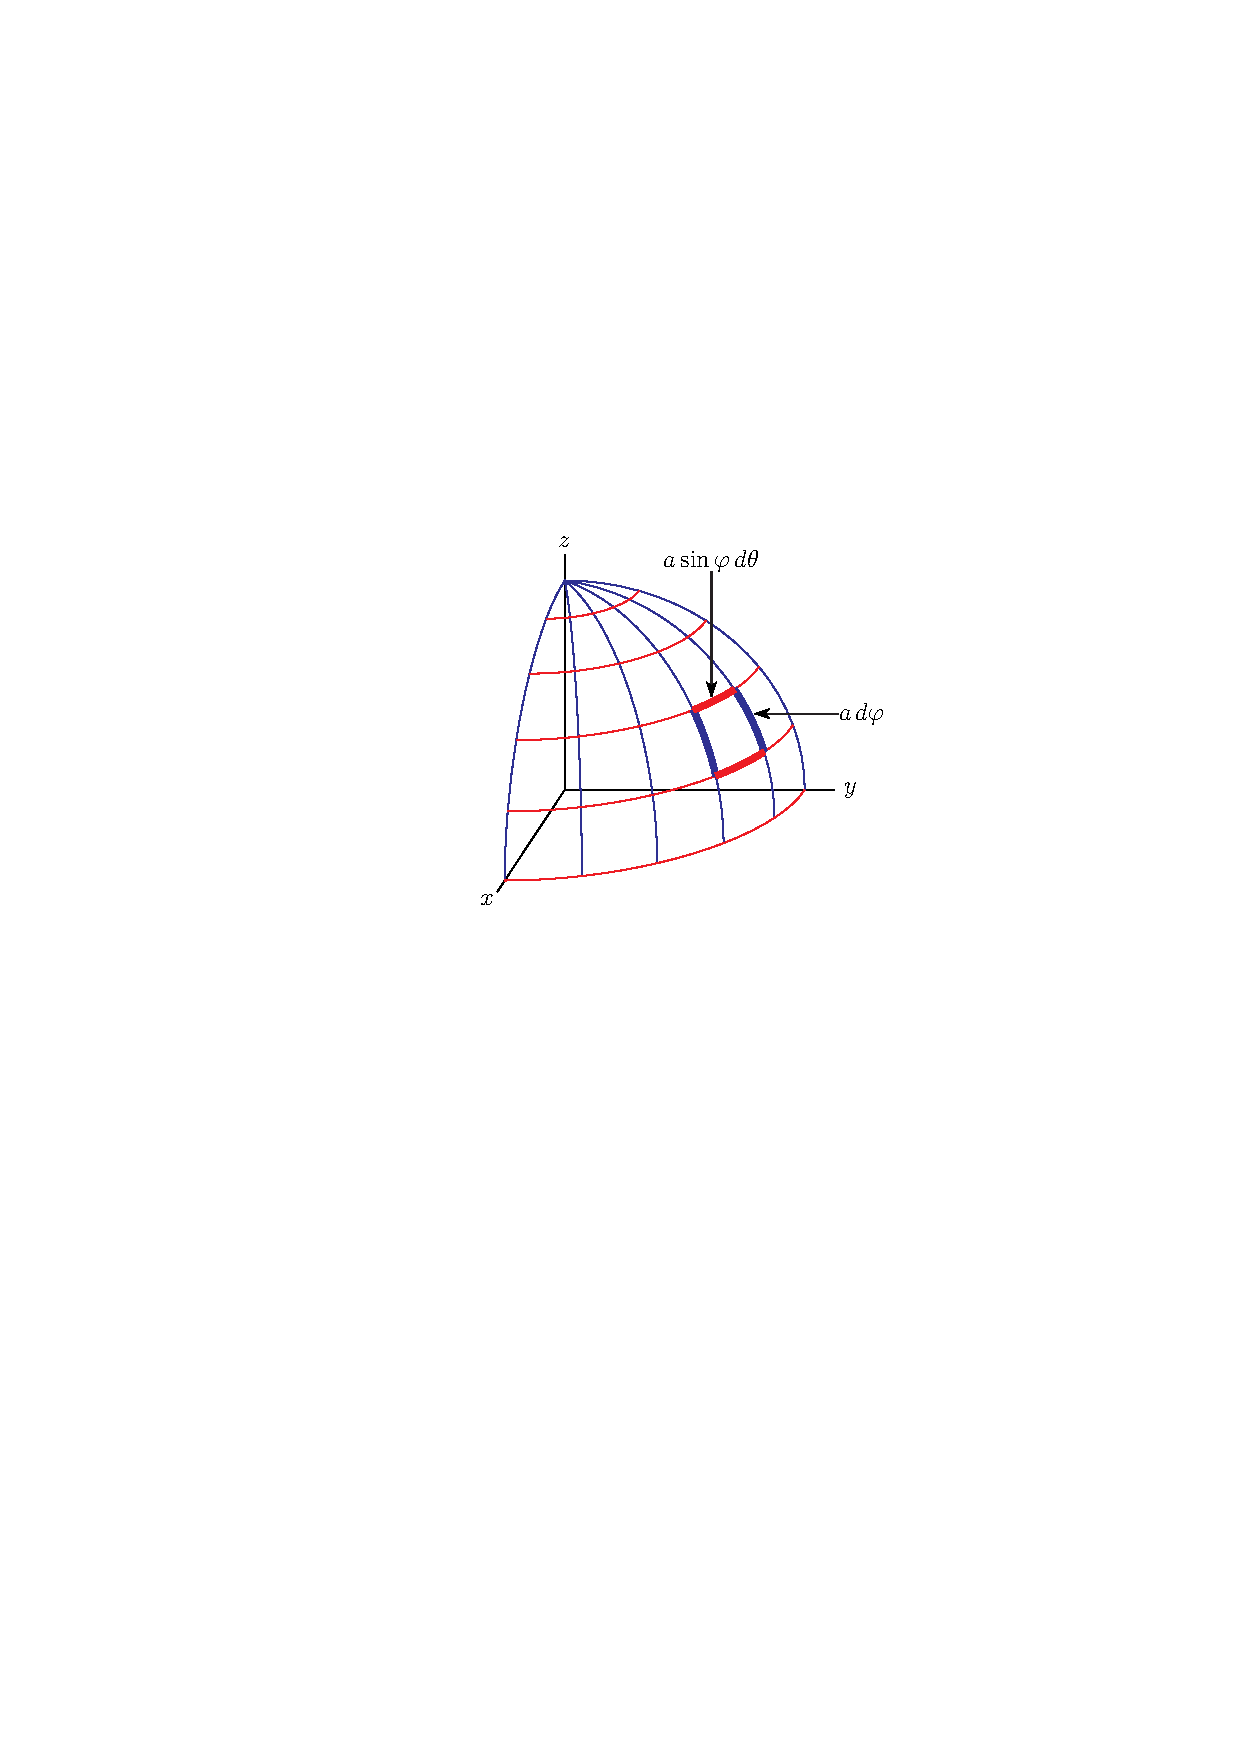
\includegraphics{sphericaldSA.pdf}
\end{center}
\end{nfig}
}
Each piece is approximately a little rectangle. Concentrate on one of them,
like the piece with the thick sides in the figure above. The area, $\dee{S}$,
of that piece is (essentially) the product of its height and its width.
Each of the two sides of the piece is
\begin{itemize}\itemsep1pt \parskip0pt \parsep0pt %\itemindent-15pt
\item[$\circ$]
a segment of a circle of radius $a$
(a fat blue line in both the figure above and in the figure on the left below) 
\item[$\circ$]
that subtends an angle $\dee{\varphi}$
\item[$\circ$]
and hence is the fraction $\frac{\dee{\varphi}}{2\pi}$ of a full circle
of radius $a$ and hence is of length 
$\frac{\dee{\varphi}}{2\pi} 2\pi a = a\dee{\varphi}$.
\end{itemize}
The top of the piece is
\begin{itemize}\itemsep1pt \parskip0pt \parsep0pt %\itemindent-15pt
\item[$\circ$]
a segment of a circle of radius $a\sin\varphi$ (a fat red line in 
both the figure above and in the figure on the right below) 
\item[$\circ$]
that subtends an angle $\dee{\theta}$
\item[$\circ$]
and hence is the fraction $\frac{\dee{\theta}}{2\pi}$ of a full circle
of radius $a\sin\varphi$ and hence is of length 
$\frac{\dee{\theta}}{2\pi} 2\pi a\sin\varphi = a\sin\varphi\dee{\theta}$.
\end{itemize}
These are drawn in the figure below.
\begin{efig}
\begin{center}
    \includegraphics{sphericaldSB.pdf}\qquad
    \includegraphics{sphericaldSC.pdf}
\end{center}
\end{efig}
So the area of our piece is 
\begin{equation*}
\dee{S} = \big(a\dee{\varphi}\big)\big(a\sin\varphi\dee{\theta}\big)
= a^2\sin\varphi\,\dee{\theta}\dee{\varphi}
\end{equation*}
This is exactly the same formula that we found for $\dee{S}$ in
Example \ref{eg:SphereAreaSC} so that we will, yet again, get that the
area of a hemisphere of radius $a$ is $2\pi a^2$. (Phew!)
\end{eg}

But wait! We can do it again, by yet another method!
\begin{eg}[Area of a hemisphere --- using $z=f(x,y)$]
       \label{eg:SphereGraph}
We'll compute the area of the hemisphere one last time\footnote{We promise!}. This time
we'll use that the equation of the hemisphere is 
\begin{equation*}
z=f(x,y) = \sqrt{a^2-x^2-y^2} 
\qquad\text{with $(x,y)$ running over $x^2+y^2\le a^2$}
\end{equation*}
So \eqref{eq:SUdSgraph} yields
\begin{align*}
\dee{S}&= \sqrt{1 + f_x(x,y)^2 + f_y(x,y)^2}\  \dee{x}\dee{y} \\
   &=\sqrt{1+\Big(\frac{-x}{\sqrt{a^2-x^2-y^2}}\Big)^2
            +\Big(\frac{-y}{\sqrt{a^2-x^2-y^2}}\Big)^2} \ \dee{x}\dee{y} \\
   &=\sqrt{1+\frac{x^2+y^2}{a^2-x^2-y^2}} \ \dee{x}\dee{y} \\
   &=\sqrt{\frac{a^2}{a^2-x^2-y^2}} \ \dee{x}\dee{y} 
\end{align*}
So the area is
$
\dblInt_{x^2+y^2\le a^2}\frac{a}{\sqrt{a^2-x^2-y^2}}
            \ \dee{x}\dee{y} 
$. We already found, in Example \ref{eg:SphereImplicit}, that the value 
of this integral in $2\pi a^2$.
\end{eg}

Let's do some more substantial examples, where the integrand is not 1.
\begin{eg}\label{eg:surfaceIntegralA}
\noindent\textit{Problem}: Evaluate
$\ \dblInt_S x^2y^2z^2\ dS\ $ where
$S$ is the part of the cone $x^2+y^2=z^2$ with $0\le z\le 1$.
\medskip
\noindent\textit{Solution 1}. 
We can express $S$ as
\begin{equation*}
z=f(x,y) = \sqrt{x^2+y^2}\qquad
x^2+y^2\le 1
\qquad \raisebox{-30pt}[20pt][25pt]{\smash{\includegraphics{coneB.pdf}}}
\end{equation*}
Now since
\begin{equation*}
f_x(x,y) = \frac{x}{\sqrt{x^2+y^2}}\qquad
f_y(x,y) = \frac{y}{\sqrt{x^2+y^2}}
\end{equation*}
\eqref{eq:SUdSgraph} gives\footnote{This answer for $\dee{S}$ is a very 
clean. Think about why. Hint: review the discussion following
\eqref{eq:SUdSgraph}.}
\begin{equation*}
\dee{S} = \Big[1 + \frac{x^2}{x^2+y^2}  + \frac{y^2}{x^2+y^2}\Big]^{1/2}
             \ \dee{x}\dee{y}
=\sqrt{2}\,\dee{x}\dee{y}
\end{equation*}
Our integral is then
\begin{align*}
\dblInt_S x^2y^2z^2\ dS
&=\sqrt{2}\dblInt_{x^2+y^2\le 1} x^2 y^2 (x^2+y^2)\ \dee{x}\dee{y}
\end{align*}
Since we are integrating over a circular domain, let's
convert to polar coordinates.
\begin{align*}
\dblInt_S x^2y^2z^2\ dS
&=\sqrt{2}\int_0^{2\pi}\dee{\theta}\int_0^1 \dee{r} \ 
          r(r\cos\theta)^2(r\sin\theta)^2 r^2 \\
&=\sqrt{2} \left[\int_0^{2\pi}\dee{\theta}\ \cos^2\theta \sin^2\theta\right]
           \left[\int_0^1 \dee{r} \ r^7\right] \\
&=\frac{\sqrt{2}}{8} \int_0^{2\pi}\dee{\theta}\ 
          \cos^2\theta \sin^2\theta 
=\frac{\sqrt{2}}{32} \int_0^{2\pi}\dee{\theta}\ \sin^2(2\theta) \\
&=\frac{\sqrt{2}}{64}  \int_0^{2\pi}\dee{\theta}\ \big[1-\cos(4\theta)\big] \\
\end{align*}
Remembering\footnote{If you have forgotten why, sketch the graph.} that the integral of $\cos(\theta)$, or $\cos(4\theta)$,
over a full period is $0$, we end up with
\begin{equation*}
\dblInt_S x^2y^2z^2\ dS = \frac{\sqrt{2}}{64}(2\pi)
   =\frac{\pi\sqrt{2}}{32} 
\end{equation*}

\medskip
\noindent\textit{Solution 2}.
We may parametrize\footnote{We did so previously, with different variable names, in Example \ref{eg:tangentPlaneA}.} the cone by
\begin{align*}
\vr(z,\theta) &= z\cos\theta\,\hi +  z\sin\theta\,\hj + z\,\hk \qquad
0\le z\le 1,\ 0\le\theta\le 2\pi
\end{align*}
Then because
\begin{align*}
\frac{\partial\vr}{\partial z}
   =  \cos\theta\,\hi +  \sin\theta\,\hj + \hk \qquad\text{and}\qquad
\frac{\partial\vr}{\partial\theta}
   =  -z\sin\theta\,\hi +  z\cos\theta\,\hj 
\end{align*}
\eqref{eq:SUdSparam} yields\footnote{Again the formula for $\dee{S}$ is
   very neat. Think about why.}
\begin{align*}
\hn\,\dee{S}
&=\pm\det\left[\begin{matrix}
                   \hi & \hj & \hk \\
                   \cos\theta & \sin\theta & 1 \\
                   -z\sin\theta & z\cos\theta & 0
                \end{matrix}\right]\,\dee{z}\dee{\theta} \\
&=\pm\big[-z\cos\theta\,\hi - z\sin\theta\,\hj + z\,\hk\big]\ 
          \dee{z}\dee{\theta} \\
\dee{S}&= \sqrt{2} z\ \dee{z}\dee{\theta}
\end{align*}
So our integral becomes
\begin{align*}
\dblInt_S x^2y^2z^2\ dS 
&= \sqrt{2}\int_0^{2\pi}\dee{\theta} \int_0^1\dee{z}\ 
           z (z\cos\theta)^2 (z\sin\theta)^2 z^2 \\
&= \sqrt{2}\int_0^{2\pi}\dee{\theta} \int_0^1\dee{z}\ z^7
           \cos^2\theta \sin^2\theta \\
&=\frac{\sqrt{2}}{8} \int_0^{2\pi}\dee{\theta}\ 
          \cos^2\theta \sin^2\theta 
\end{align*} 
We evaluated this integral in Solution 1. So again
\begin{equation*}
\dblInt_S x^2y^2z^2\ dS   =\frac{\pi\sqrt{2}}{32} 
\end{equation*}
\end{eg}

Let's do something more celestial.
\begin{eg}\label{eg:surfaceIntegralB}
Consider a spherical shell of radius $a$ with mass density $\mu$ per unit
area. Think of it as a hollow planet\footnote{A favourite of science 
fiction and fantasy writers. Plug ``subterranean fiction'' into your favourite
search engine. While you're at it, also try ``gravity train''. We'll look at it in the optional Example \ref{eg:gravityTrain}.}.
We are going to determine the gravitational force that it exerts on a particle
of mass $m$ a distance $b$ away from its centre. This particle can be either
outside the shell ($b>a$) or inside the shell ($b<a$).
We can choose the coordinate system so that the centre of the shell is at the origin and the particle is
at $(0,0,b)$. By Newton's law of gravitation, the force exerted on the 
particle by a tiny piece of the shell of surface area $\dee{S}$ located at $\vr$ is
\begin{equation*}
\frac{G\,(\mu\dee{S})\,m}{|\vr-(0,0,b)|^3}(\vr-(0,0,b))
\end{equation*} 
Here $G$ is the gravitational constant, $\mu\dee{S}$ is the mass of the tiny
piece of shell, $m$ is the mass of the particle 
\vadjust{
\begin{efig}
\begin{center}
    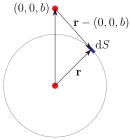
\includegraphics{shell.pdf}\qquad
    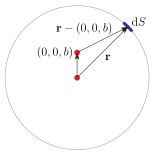
\includegraphics{shellB.pdf}\qquad
\end{center}
\end{efig}
}
and $\vr-(0,0,b)$ is the vector from the
particle to the piece of shell. If we work in spherical coordinates, as we did in Example \ref{eg:SphereAreaSC},
\begin{align*}
\dee{S} &= a^2\sin\varphi\,\dee{\varphi}\dee{\theta} 
\end{align*}
and
\begin{align*}
\vr &= a\sin\varphi\cos\theta\,\hi 
      + a\sin\varphi\sin\theta\,\hj 
      + a\cos\varphi\,\hk \\
\vr-(0,0,b) &= a\sin\varphi\cos\theta\,\hi 
      + a\sin\varphi\sin\theta\,\hj 
      + (a\cos\varphi-b)\,\hk  \\
|\vr-(0,0,b)|^2 &= a^2+b^2 -2ab\cos\varphi 
\end{align*}
The total force is then
\begin{align*}
\vF = 
    G\mu m a^2\int_0^\pi\dee{\varphi} \int_0^{2\pi}\dee{\theta}\ \sin\varphi\ 
    \frac{a\sin\varphi\cos\theta\,\hi 
      + a\sin\varphi\sin\theta\,\hj 
      + (a\cos\varphi-b)\,\hk}
         {\big[a^2+b^2 -2ab\cos\varphi\big]^{3/2}}
\end{align*}
Note for future reference that the square root in
$[a^2+b^2 -2ab\cos\varphi]^{3/2}$ is the \emph{positive}
square root because $[b^2+a^2 -2ab\cos\varphi]^{1/2}$ is the length
of $\vr-(0,0,b)$, which is positive. 

This integral is a little different than other integrals that we have 
encountered so far in that the integrand is a vector. By 
definition\footnote{Under this definition we still have 
$\dblInt (\vA+\vB)\,\dee{S} = \dblInt \vA\,\dee{S} + \dblInt\vB\,\dee{S}$.
},
\begin{equation*}
\dblInt_S \big[G_1\,\hi + G_2\,\hj + G_3\,\hk \big]\ \dee{S}
=\hi \dblInt_S G_1\ \dee{S}
+\hj \dblInt_S G_2\ \dee{S}
+\hk \dblInt_S G_3\ \dee{S}
\end{equation*}
so we just have to compute the three components separately. 

In our case,
the $\hi$ and $\hj$ components 
\begin{align*}
\vF\cdot\hi & = G\mu m a^2 \int_0^\pi\dee{\varphi} \left[
\sin\varphi\ 
    \frac{a\sin\varphi}
         {\big[a^2+b^2 -2ab\cos\varphi\big]^{3/2}}
\int_0^{2\pi}\dee{\theta}\ \cos\theta
\right] \\
\vF\cdot\hj & = G\mu m a^2\int_0^\pi\dee{\varphi}\left[
 \sin\varphi\ 
    \frac{a\sin\varphi}
         {\big[a^2+b^2 -2ab\cos\varphi\big]^{3/2}}
\int_0^{2\pi}\dee{\theta}\ \sin\theta
\right]
\end{align*}
are both zero\footnote{Think about why the $\hi$ and $\hj$ components
should both be zero. Think symmetry.} because
$\int_0^{2\pi}\cos\theta\ \dee{\theta}
           =\int_0^{2\pi}\sin\theta\ \dee{\theta}
           =0$
so that
\begin{align*}
\vF 
&=  G\mu m a^2 \hk\int_0^\pi\dee{\varphi} \int_0^{2\pi}\dee{\theta}\ \sin\varphi\ 
    \frac{a\cos\varphi-b}
         {\big[a^2+b^2 -2ab\cos\varphi\big]^{3/2}} \\
&=  2\pi G\mu m a^2 \hk\int_0^\pi\dee{\varphi}\ \sin\varphi\ 
    \frac{a\cos\varphi-b}
         {\big[a^2+b^2 -2ab\cos\varphi\big]^{3/2}}
\end{align*}
To evaluate this integral we substitute
\begin{align*}
u=a^2+b^2 -2ab\cos\varphi\qquad
\dee{u} = 2ab\sin\varphi\,\dee{\varphi}\qquad
\cos\varphi = \frac{a^2+b^2-u}{2ab}
\end{align*}
When $\varphi=0$, $u=(a-b)^2$ and when $\varphi =\pi$, $u=(a+b)^2$, so
\begin{align*}
\vF 
&=  \frac{\pi G\mu m a}{b} \hk\int_{(a-b)^2}^{(a+b)^2} 
     \dee{u}\  \frac{\frac{a^2+b^2-u}{2b}-b}  {u^{3/2}} \\
&=  \frac{\pi G\mu m a}{b} \hk\int_{(a-b)^2}^{(a+b)^2} 
     \dee{u}\  \frac{\frac{a^2-b^2-u}{2b}}  {u^{3/2}} \\
&=  \frac{\pi G\mu m a}{b} \hk\Big[ 
      \Big(\frac{a^2-b^2}{2b}\Big)\frac{u^{-1/2}}{-1/2}
            -\Big(\frac{1}{2b}\Big)\frac{u^{1/2}}{1/2}
   \Big]_{(a-b)^2}^{(a+b)^2}
\end{align*}
Recalling that $u^{1/2}$ is the \emph{positive} square root,
\begin{align*}
\vF&=\frac{\pi G\mu m a}{b} \hk\Big[ 
      \Big(\frac{b^2-a^2}{b}\Big)\frac{1}{a+b}
            -\frac{a+b}{b}
            -\Big(\frac{b^2-a^2}{b}\Big)\frac{1}{|a-b|}
            +\frac{|a-b|}{b}
   \Big]
\end{align*}
If $b>a$, so that $|a-b|=b-a$
\begin{align*}
\vF&=\frac{\pi G\mu m a}{b} \hk\Big[ 
       \frac{b-a}{b}
            -\frac{a+b}{b}
            -\frac{a+b}{b}
            +\frac{b-a}{b}
   \Big]
=-\frac{G(4\pi a^2\mu)m}{b^2} \hk
\end{align*}
If $b<a$, so that $|a-b|=a-b$
\begin{align*}
\vF&=\frac{\pi G\mu m a}{b} \hk\Big[ 
      \frac{b-a}{b}
            -\frac{a+b}{b}
            +\frac{a+b}{b}
            +\frac{a-b}{b}
   \Big]
=0
\end{align*}
The moral\footnote{These two results appeared in Isaac Newton's
Principia Mathematica (1687). They are known as Newton's ``superb 
theorems''.} is
\begin{itemize}
\item[$\circ$] 
if the particle is inside the shell, it feels no gravitational force at all,
and
\item[$\circ$]
if the particle is outside the shell, it feels the same gravitational force
as it would if the entire mass of the shell ($4\pi a^2\mu$) were
concentrated at the centre of the shell.
\end{itemize}
%So, for many purposes, a planet can be thought of as a point particle.
\end{eg}

\begin{eg}[Optional --- Gravity Train]\label{eg:gravityTrain}
The ``Gravity Train\footnote{The British physicist and architect
(he was Surveyor to the City of London and chief assistant to Christopher Wren) Robert Hooke (1635--1703) wrote about the gravity train idea in a letter to Isaac Newton. A gravity train was used in the 2012 movie 
\emph{Total Recall}.}'' refers to the following curious, though admittedly
not very practical, thought experiment.

\begin{itemize}
\item
Pretend that the Earth is a perfect sphere of radius $R$ and that 
it has a constant mass density $\rho$.

\item 
Pick \emph{any} two distinct points on the surface of the Earth. Call
them $V$ and $M$.

\item
Bore a tunnel straight through the Earth from $V$ to $M$.

\item
Place a train in the tunnel at $V$. Assume that the only forces acting
on the train are gravity, $\vG$, and a normal force, $\vN$, that  the tunnel
imposes on the train to keep it in the tunnel. In particular, there are 
no frictional forces, like air resistance, and the train does not
have an engine. Release the train and assume that it does not melt 
as it passes through the centre of the Earth.

\end{itemize}

\begin{nfig}
\begin{center}
    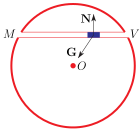
\includegraphics{gravityTrain.pdf}
\end{center}
\end{nfig}
What happens?

We'll simplify our analysis of the motion of the train by 
picking a convenient coordinate system. 
\begin{itemize}\itemsep1pt \parskip0pt \parsep0pt %\itemindent-15pt
\item[$\circ$]
First translate our coordinate system so that the centre of the
Earth, call it $O$, is at the origin, $(0,0,0)$.
\item[$\circ$]
Then rotate our coordinate system about the origin so that the origin,
$V$ and $M$ all lie in the $xz$-plane.
\item[$\circ$]
Then rotate our coordinate system about the $y$-axis so that $V$ and $M$
have the same $z$-coordinate $Z\ge 0$. So the coordinates of $V$ and $M$
are $\big(\pm\sqrt{R^2-Z^2}\,,\,0\,,Z\big)$. Let's suppose that $V$ is
at $\big(\sqrt{R^2-Z^2}\,,\,0\,,Z\big)$ and $M$ is at
$\big(-\sqrt{R^2-Z^2}\,,\,0\,,Z\big)$. It really doesn't matter which is which,
but we can always arrange that it is $V$ at 
$\big(+\sqrt{R^2-Z^2}\,,\,0\,,Z\big)$ by rotating around the
$z$-axis by $180^\circ$ if necessary.

\end{itemize}

\begin{nfig}
\begin{center}
    \includegraphics{gravityTrainB.pdf}
\end{center}
\end{nfig}
The $y$- and $z$-coordinates of the train are always fixed at $0$ and 
$Z$, respectively. So let's call the $x$-coordinate at time $t$
$x(t)$, and look at the $x$-component of Newton's law of motion.
\begin{align*}
m\va = \vG +\vN
\end{align*} 
It is
\begin{equation*}
m x''(t) = \vG\cdot\hi
\end{equation*}
because the normal force $\vN$ has no $\hi$ component. Recall that 
Newton's law of gravity says that
\begin{equation*}
\vG = -\frac{GMm}{|\vr|^3}\vr
\end{equation*}
where $G$ is the gravitational constant, $\vr$ is the vector from $O$ to the train, and $m$ is the mass of the train. In this case, because of our 
computation in Example \ref{eg:surfaceIntegralB}, the train only feels 
gravity from shells of the Earth that are inside the train, so that
$M$ is the mass of the 
\vadjust{
\begin{nfig}
\begin{center}
    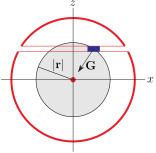
\includegraphics{gravityTrainC.pdf}
\end{center}
\end{nfig}
}
part of the Earth whose distance to the centre of the Earth is no more 
than $|\vr|$. So
\begin{equation*}
M = \frac{4}{3}\pi |\vr|^3\rho
\end{equation*}
and
\begin{equation*}
mx''(t) = -\frac{Gm}{|\vr|^3}\  \frac{4}{3}\pi |\vr|^3\rho\ \vr\cdot\hi
\end{equation*}
so that
\begin{equation*}
x''(t) + \frac{4\pi G\rho}{3} x(t) = 0
\end{equation*}
This is exactly the differential equation of simple harmonic motion.
We have seen it before in Example \ref{eg:vortexStreamEqual}.
Except for the constant $\frac{4\pi G\rho}{3}$, it is identical to the
equation solved in Example \ref{exBVP} of the Appendix \ref{ap:ODE}, entitled
``Review of Linear Ordinary Differential Equations''. 
The general solution is
\begin{equation*}
x(t)  = C_1 \cos\left(\sqrt{\frac{4\pi G\rho}{3}}\ t\right) 
             +  C_2 \sin\left(\sqrt{\frac{4\pi G\rho}{3}}\ t\right) 
\end{equation*}
with $C_1$ and $C_2$ being arbitrary constants. If we release the train, 
from rest, at $t=0$, then $x(0) = \sqrt{R^2-Z^2}$ and $x'(0)=0$
so that $C_1= \sqrt{R^2-Z^2}$, $C_2=0$ and
\begin{equation*}
x(t)  = \sqrt{R^2-Z^2} \cos\left(\sqrt{\frac{4\pi G\rho}{3}}\ t\right) 
\end{equation*}
The train reaches $M$ when $x(t)  = -\sqrt{R^2-Z^2}$. That is, when
$\cos\left(\sqrt{\frac{4\pi G\rho}{3}}\ t\right)=-1$. So the transit
time, $T$, from $V$ to $M$ obeys
\begin{equation*}
\sqrt{\frac{4\pi G\rho}{3}}\ T=\pi
\implies
T= \pi  \sqrt{\frac{3}{4\pi G\rho}}
  = \sqrt{\frac{3\pi}{4 G\rho}}
\end{equation*}
Notice that this transit time depends only on the gravitational constant
$G$ and the density of the Earth $\rho$. In particular it is 
completely independent of  
\begin{itemize}\itemsep1pt \parskip0pt \parsep0pt %\itemindent-15pt
\item[$\circ$]
where $V$ and $M$ are and, in particular, 
\item[$\circ$]
how close together $V$ and $M$ are, and also of
\item[$\circ$]
the radius of the Earth.
\end{itemize}
In the case of the Earth, the transit time is about 42 minutes.

\intremark{
\begin{align*}
G&=6.67\times 10^{-11}\  {\rm m}^3\  {\rm kg}^{-1}\ {\rm sec}^{-2}
\\
\rho&=5.51\ {\rm g}\ {\rm cm}^{-3} 
     =5.51\times 10^{-3+6}\ {\rm kg}\ {\rm m}^{-3}
\\
G\rho & = 36.75\times 10^{-8}\ {\rm sec}^{-2}
\\
\sqrt{\frac{3\pi}{4 G\rho}} & = 0.253\times 10^4\ {\rm sec} = 42.2\ {\rm min}
\end{align*}
}

\end{eg}



\subsection{Optional --- Dropping Higher Order Terms in $\dee{u},\dee{v}$}\label{sec:hoterms}
In the course of deriving \eqref{eq:SUdSparam}, that is,
$\hn\dee{S}$ and $\dee{S}$ formulae for 
\begin{nfig}
\begin{center}
    \includegraphics{dS.pdf}
\end{center}
\end{nfig}
we approximated, for example, the vectors
\begin{alignat*}{3}
\overrightarrow{P_0P_1}
&=\vr(u_0+\dee{u}, v_0) -\vr(u_0\,,\,v_0) 
&= \frac{\partial\vr}{\partial u}(u_0\,,\,v_0)\,\dee{u} + E_1
&\approx \frac{\partial\vr}{\partial u}(u_0\,,\,v_0)\,\dee{u}  \\[0.1in]
\overrightarrow{P_0P_2}
&=\vr(u_0, v_0+\dee{v})-\vr(u_0\,,\,v_0) 
&= \frac{\partial\vr}{\partial v}(u_0\,,\,v_0)\,\dee{v}  + E_2
&\approx \frac{\partial\vr}{\partial v}(u_0\,,\,v_0)\,\dee{v}  
\end{alignat*}
where $E_1$ is bounded\footnote{Remember the error in the Taylor polynomial 
approximations.} by a constant times $\dee{u}^2$
and $E_2$ is bounded by a constant times $\dee{v}^2$. That is, we assumed 
that we could just drop $E_1$ and $E_2$. 

So we approximated
\begin{align*}
\big|\overrightarrow{P_0P_1}\times\overrightarrow{P_0P_2}\big|
&=\Big|\Big[\frac{\partial\vr}{\partial u}(u_0\,,\,v_0)\,\dee{u} + E_1\Big]
\times\Big[\frac{\partial\vr}{\partial v}(u_0\,,\,v_0)\,\dee{v} + E_2\Big]
\Big| \\
&=\Big|\frac{\partial\vr}{\partial u}(u_0\,,\,v_0)\,\dee{u} 
\times\frac{\partial\vr}{\partial v}(u_0\,,\,v_0)\,\dee{v} + E_3
\Big| \\
&\approx \Big|\frac{\partial\vr}{\partial u}(u_0\,,\,v_0)\,\dee{u} 
\times\frac{\partial\vr}{\partial v}(u_0\,,\,v_0)\,\dee{v}
\Big|
\end{align*}
where the length of the vector $E_3$ is bounded by a constant times 
$\dee{u}^2\,\dee{v}+\dee{u}\,\dee{v}^2$.
We'll now see why dropping terms like $E_3$ does not change the value
of the integral at all\footnote{See the optional \S 1.1.6 of the CLP-2 text
for an analogous argument concerning Riemann sums.}. 

Suppose that our domain of integration consists of all $(u,v)$'s 
in a rectangle of width $A$ and height $B$, as in the figure below.
\vadjust {
\begin{nfig}
\begin{center}
    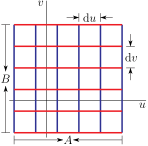
\includegraphics{slicing.pdf}
\end{center}
\end{nfig}
}
Subdivide the rectangle into a grid of $n\times n$ small subrectangles 
by drawing lines of constant $v$ (the red lines in the figure) and 
lines of constant $v$ (the blue lines in the figure).
Each subrectangle has width $\dee{u} = \frac{A}{n}$ and height
$\dee{v} = \frac{B}{n}$. Now suppose that in setting up the integral 
we make, for each subrectangle, an error that is bounded by some constant
times
\begin{equation*}
\dee{u}^2\,\dee{v}+\dee{u}\,\dee{v}^2
=\Big(\frac{A}{n}\Big)^2 \frac{B}{n}
 +  \frac{A}{n}\Big(\frac{B}{n}\Big)^2
=\frac{AB(A+B)}{n^3}
\end{equation*}
Because there are a total of $n^2$ subrectangles, the total error that 
we have introduced, for all of these subrectangles, is no larger than 
a constant times
\begin{equation*}
n^2 \times \frac{AB(A+B)}{n^3} = \frac{AB(A+B)}{n}
\end{equation*}
When we define our integral by taking the limit $n\rightarrow 0$ of 
the Riemann sums, this error converges to exactly $0$.


\section{Interpretation of Flux Integrals}\label{sec:fluxIntegrals}

We defined, in \S\ref{sec:surfaceIntegrals}, two types of integrals 
over surfaces. We have seen, in \S\ref{sec:rhodSexamples}, some
applications that lead to integrals of the type 
$\dblInt_S \rho\,\dee{S}$. We now look at one application that leads 
to integrals of the type $\dblInt_S \vF\cdot\hn\,\dee{S}$. Recall
that integrals of this type are called flux integrals. Imagine a fluid
with 
\begin{itemize}
\item
the density of the fluid (say in kilograms per cubic meter) at position
$(x,y,z)$ and time $t$ being $\rho(x,y,z,t)$ and with

\item
the velocity of the fluid  (say in meters per second) at position
$(x,y,z)$ and time $t$ being $\vv(x,y,z,t)$. 
\end{itemize}
We are going to determine the rate (say in kilograms per second) 
at which the fluid is flowing through a tiny piece $\dee{S}$ of surface 
at $(x,y,z)$. During a tiny time interval of length $\dee{t}$ about
time $t$, fluid near $\dee{S}$ moves $\vv(x,y,z,t)\dee{t}$. The green
line in the figure below is a side view of $\dee{S}$ and $\hn=\hn(x,y,z)$ is a unit 
normal vector to $\dee{S}$.
\vadjust{
\begin{nfig}
\begin{center}
    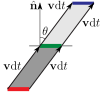
\includegraphics{fluxIntDeriv.pdf}
\end{center}
\end{nfig}
}
So during that tiny time interval
\begin{itemize}\itemsep1pt \parskip0pt \parsep0pt %\itemindent-15pt
\item[$\circ$] the red line moves to the green line and
\item[$\circ$] the green line moves to the blue line so that
\item[$\circ$] the fluid filling the dark grey region below the green line
crosses through $\dee{S}$ and moves to light grey region above the green line.
\end{itemize}
If we denote by $\theta$ the angle between $\hn$ and $\vv\dee{t}$,
\begin{itemize}\itemsep1pt \parskip0pt \parsep0pt %\itemindent-15pt
\item[$\circ$] 
the volume of fluid that crosses through $\dee{S}$ during the time 
interval $\dee{t}$ is the volume  whose side view is the dark grey 
region below the green line. This region has base $\dee{S}$ and 
height $|\vv\dee{t}|\cos\theta$ and so has volume
\begin{equation*}
|\vv(x,y,z,t)\dee{t}|\cos\theta\ \dee{S}
   =\vv(x,y,z,t)\cdot\hn(x,y,z)\,\dee{t}\,\dee{S}
\end{equation*}
because $\hn(x,y,z)$ has length one. 
\item[$\circ$]
 The mass of fluid that crosses $\dee{S}$ during the time interval $\dee{t}$
 is then 
\begin{equation*}
\rho(x,y,z,t)\vv(x,y,z,t)\cdot\hn(x,y,z)\,\dee{t}\,\dee{S}
\end{equation*}
\item[$\circ$]
and the rate at which fluid is crossing through $\dee{S}$ is
\begin{equation*}
\rho(x,y,z,t)\vv(x,y,z,t)\cdot\hn(x,y,z)\,\dee{S}
\end{equation*}
\end{itemize}
Integrating $\dee{S}$ over a surface $S$, we conclude that
\begin{lemma}\label{lem:fluxInterp}
The rate at which fluid mass is crossing through a surface $S$ is the flux integral
\begin{align*}
\dblInt_S \rho(x,y,z,t)\vv(x,y,z,t)\cdot\hn(x,y,z)\,\dee{S}
\end{align*}
Here $\rho$ is the density of the fluid, $\vv$ is
the velocity field of the fluid, and $\hn(x,y,z)$ is a unit normal 
to $S$ at $(x,y,z)$.
If the flux integral is positive the fluid is crossing in the direction 
$\hn$. If it is negative the fluid is crossing opposite to the direction 
of~$\hn$. The rate at which volume of fluid is crossing through a surface $S$ is the flux integral
\begin{align*}
\dblInt_S \vv(x,y,z,t)\cdot\hn(x,y,z)\,\dee{S}
\end{align*}
\end{lemma}

%%%%%%%%%%%%%%%%%%%%%%%%%%%%%%%%%%%%%%%%%%%%%%%%%%%%%%
\subsection{Examples of Flux Integrals}\label{sec:fluxEexamples}

\begin{eg}[Point Source]\label{eg:fluxIntegralA}
In Example \ref{eg:ptSource}, we found that the vector field of
a point source\footnote{You can imagine that a very small pipe pumps water to
the origin.} (in three dimensions) that creates $4\pi m$ liters per second 
is
\begin{equation*}
\vv(x,y,z) = \frac{m}{r(x,y,z)^2}\,\hat\vr(x,y,z)
\end{equation*}
where
\begin{equation*}
r(x,y,z) = \sqrt{x^2+y^2+z^2}\qquad
\hat\vr(x,y,z) = \frac{x\hi + y\hj + z\hk}{\sqrt{x^2+y^2+z^2}}
\end{equation*}
We sketched it in Figure \ref{fig:sourceField}.
We'll now compute the flux of this vector field across a
sphere centred on the origin. Suppose that the sphere has radius $R$.
\vadjust{
\begin{nfig}
\begin{center}
    \includegraphics{sourceFlux.pdf}
\end{center}
\end{nfig}
}
Then the outward\footnote{It doesn't really matter which unit normal we pick here. We just have to be clear which one we're using. With the outward normal,
the flux gives the rate at which fluid crosses the sphere in the outward 
direction. If we were to use the inward pointing normal, the flux 
would give the rate at which fluid crosses the sphere in the inward 
direction.
} pointing normal at a point $(x,y,z)$ on the sphere is
\begin{equation*}
\hn(x,y,z) = \hat\vr(x,y,z) = \frac{x\hi + y\hj + z\hk}{\sqrt{x^2+y^2+z^2}}
= \frac{x\hi + y\hj + z\hk}{R}
\end{equation*}
Note that $\hat\vr(x,y,z)\cdot \hat\vr(x,y,z)=1$ and that, on the sphere,
$r(x,y,z)=R$.
So the flux of $\vv$ outward through the sphere is
\begin{align*}
 \dblInt_S\vv\cdot\hn\ \dee{S}
&= \dblInt_S \frac{m}{r(x,y,z)^2}\,\hat\vr(x,y,z) \cdot \hat\vr(x,y,z)\ \dee{S}
\\
&= \dblInt_S \frac{m}{R^2}\ \dee{S}
=\frac{m}{R^2} 4\pi R^2
\\
&=4\pi m
\end{align*}
This is the rate at which volume of fluid is exiting the sphere.
In our derivation of the vector field we assumed that the fluid is
incompressible, so it is also the rate at which the point source is 
creating fluid.

\end{eg}


\begin{eg}[Vortex]\label{eg:fluxIntegralB}
In Figure \ref{fig:vortexField}, we sketched the vector field
(in two dimensions)
\begin{equation*}
\vv(x,y) = \Om\big(-y\hi +x\hj\big)
\end{equation*}
We'll now compute the flux of this vector field across a
circle $C$ centred on the origin. Suppose that the circle has radius $R$.
\vadjust{
\begin{nfig}
\begin{center}
    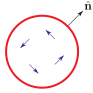
\includegraphics{vortexFlux.pdf}
\end{center}
\end{nfig}
}
By definition, in two dimensions, the flux of a vector field across a curve
$C$ is $\int_C\vv\cdot\hn\ \dee{s}$. 

This is the natural analog of the
flux in three dimensions --- the surface $S$ has been replaced by the 
curve $C$, and the surface area $\dee{S}$ of a tiny piece of $S$ has been
replaced by the arc length $ds$ of a tiny piece of $C$.

The outward pointing unit normal at a point $(x,y)$ on our circle $C$ is
\begin{equation*}
\hn(x,y) = \frac{x\hi + y\hj}{\sqrt{x^2+y^2}}
= \frac{x\hi + y\hj}{R}
\end{equation*}
So
\begin{equation*}
\vv(x,y)\cdot\hn(x,y)
=\frac{\Om}{R}\big(-y\hi + x\hj\big)\cdot\big(x\hi + y\hj\big)
=0
\end{equation*}
and the flux across $C$ is 
\begin{equation*}
\int_C\vv\cdot\hn\ \dee{s}=0
\end{equation*}
This should not be a surprise --- no fluid is crossing $C$ at all.
This is exactly what we would expect from looking at the arrows in
Figure \ref{fig:vortexField} or at the stream lines in Example 
\ref{eg:vortexStreamParallel}.
\end{eg}

\begin{eg}\label{eg:fluxIntegralC}
\noindent\textit{Problem}: Evaluate
$\ \dblInt_S\vF\cdot\hn\ dS\ $ where
\begin{equation*}
\vF(x,y,z) = (x+y)\,\hi + (y+z)\,\hj + (x+z)\,\hk
\end{equation*}
and $S$ is the boundary of $V=\Set{(x,y,z)}{0\le x^2+y^2\le 9,\ 0\le z\le 5}$,
and $\hn$ is the outward normal\footnote{It is necessary that the problem specify, one way or another, whether $\hn$ is the inward pointing normal or the outward pointing normal. Without this, the meaning of 
$\ \dblInt_S\vF\cdot\hn\ dS\ $ is ambiguous. Think about where the orientation of the normal vector gets used in your solution.} to $S$. 

\medskip
\noindent\textit{Solution}.
The volume $V$ looks like a tin can of radius $3$ and height $5$.
\vadjust{
\begin{nfig}
\begin{center}
    \includegraphics{cylinder1.pdf}
\end{center}
\end{nfig}
}
It is natural to decompose its surface $S$ into three parts
\begin{align*}
S_t &= \Set{(x,y,z)}{0\le x^2+y^2\le 9,\  z= 5} = \text{the top} \\
S_b &= \Set{(x,y,z)}{0\le x^2+y^2\le 9,\  z= 0} = \text{the bottom} \\
S_s &= \Set{(x,y,z)}{x^2+y^2 = 9,\  0\le z\le 5} = \text{the side} 
\end{align*}
We'll compute the flux through each of the three parts separately and 
then add them together.

\noindent\emph{The Top:}\ \ \ On the top, the outward pointing normal to
$S$ is $\hn=\hk$ and $\dee{S} = \dee{x}\dee{y}$. This is probably
intuitively obvious. But if it isn't, you can always derive it by parametrizing
the top by $\vr(x,y) = x\,\hi +y\,\hj + 5\,\hk$ with $x^2+y^2\le 9$.
So the flux through the top is
\begin{align*}
\dblInt_{S_t}\vF\cdot\hn\ \dee{S}
&= \dblInt_{\atp{x^2+y^2\le 9}{z=5}} (x+z)\ \dee{x}\dee{y}
= \dblInt_{x^2+y^2\le 9} (x+5)\ \dee{x}\dee{y}
\end{align*}
The integral $\dblInt_{x^2+y^2\le 9} x\ \dee{x}\dee{y}=0$ since $x$
is odd and the domain of integration is symmetric about $x=0$.
So 
\begin{align*}
\dblInt_{S_t}\vF\cdot\hn\ \dee{S}
= \dblInt_{x^2+y^2\le 9} 5\ \dee{x}\dee{y}
=5\pi(3)^2
=45\pi
\end{align*}


\noindent\emph{The Bottom:}\ \ \ On the bottom, the outward pointing normal to
$S$ is $\hn=-\hk$ and $\dee{S} = \dee{x}\dee{y}$. 
So the flux through the bottom is
\begin{align*}
\dblInt_{S_b}\vF\cdot\hn\ \dee{S}
&= -\dblInt_{\atp{x^2+y^2\le 9}{z=0}} (x+z)\ \dee{x}\dee{y}
= -\dblInt_{x^2+y^2\le 9} x\ \dee{x}\dee{y}
=0
\end{align*}
again since $x$ is odd and the domain of integration is symmetric about $x=0$.

\noindent\emph{The Side:}\ \ \ We can parametrize the side by
using cylindrical coordinates.
\begin{equation*}
\vr(\theta,z) = \big(3\cos\theta\,,\,3\sin\theta\,,\,z\big)\qquad
0\le\theta < 2\pi,\ 0\le z\le 5
\end{equation*}
Then, using \eqref{eq:SUdSparam}, 
\begin{align*}
\frac{\partial\vr}{\partial\theta}
&=(-3\sin\theta\,,\,3\cos\theta\,,\,0) \\
%
\frac{\partial\vr}{\partial z} &=(0\,,\,0\,,\,1)\\
%
\hn\,\dee{S}&=
\frac{\partial\vr}{\partial\theta}
\times\frac{\partial\vr}{\partial z}\ \dee{\theta}\,\dee{z}\hskip1.5in
\raisebox{-20pt}[20pt][15pt]{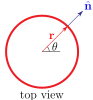
\includegraphics{canTopView.pdf}}
\\
&=(3\cos\theta\,,\,3\sin\theta\,,\,0)\ \dee{\theta}\,\dee{z}
\end{align*}
Note that $\hn = (\cos\theta\,,\,\sin\theta\,,\,0)$ is 
outward pointing\footnote{To check, draw, in your head, a sketch of the top 
view of the can. ``Top view'' just means ``ignore the $z$-coordinate''.
The top view of the can is a circle of radius $3$. Then, at a generic point,
$\vr=(\cos\theta,\sin\theta)$, on the can, draw the unit normal 
$\hn = (\cos\theta\,,\,\sin\theta)$ with its tail at $\vr$. It is pointing
away from the origin, just like $\vr$ is. That is, $\hn$ is pointing outward.},
as desired.
Continuing,
\begin{align*}
\vF\big(x(\theta,z)\,,\,y(\theta,z)\,,\,z(\theta,z)\big)
&=3(\cos\theta+\sin\theta)\ \hi
  +(3\sin\theta+z)\ \hj+(3\cos\theta+z)\ \hk\\
\vF\cdot\hn\,\dee{S}
&=\big\{9\cos^2\theta+3\sin\theta\cos\theta+9\sin^2\theta+3z\sin\theta\big\}\ 
         \dee{\theta}\,\dee{z} \\
&=\big\{9 +\nicefrac{3}{2}\,\sin(2\theta)+3z\sin\theta\big\}\ 
           \dee{\theta}\,\dee{z}
\end{align*}
 So the flux through the side is
\begin{align*}
\dblInt_{S_s}\vF\cdot\hn\ \dee{S}
&=\int_0^{2\pi}\dee{\theta}\int_0^5\dee{z}\  
     \big\{9 +\nicefrac{3}{2}\,\sin(2\theta)+3z\sin\theta\big\} \\
&=9\int_0^{2\pi}\dee{\theta}\int_0^5\dee{z}
\qquad\qquad\text{since }\int_0^{2\pi}\sin\theta\,\dee{\theta}
                   =\int_0^{2\pi}\sin(2\theta)\,\dee{\theta} 
                   =0 \\
&=9\times 2\pi\times 5 
=90\pi
\end{align*}
and the total flux is
\begin{align*}
\dblInt_{S}\vF\cdot\hn\ \dee{S}
=\dblInt_{S_t}\vF\cdot\hn\ \dee{S}
 +\dblInt_{S_b}\vF\cdot\hn\ \dee{S}
 +\dblInt_{S_s}\vF\cdot\hn\ \dee{S}
=45\pi+0+90\pi
=135\pi
\end{align*}



\end{eg}


\begin{eg}\label{eg:fluxIntegralL}
\noindent\textit{Problem}: Evaluate
$\ \dblInt_S\vF\cdot\hn\ dS\ $ where
$\ \vF(x,y,z)=x^4\hi+2y^2\hj+z\hk,\ $ $S$ is the half of the surface
$\ \frac{1}{4}x^2+\frac{1}{9}y^2+z^2=1\ $ with $z\ge 0$, and $\hn$ is the 
upward pointing unit normal. 

\begin{nfig}
\begin{center}
   \includegraphics{ellipsoid.pdf}
\end{center}
\end{nfig}

\medskip
\noindent\textit{Solution 1}.  We start by parametrizing the surface,
which is half of an ellipsoid. By way of motivation for the parametrization,
recall that spherical coordinates, with $\rho=1$,  provide a natural way to 
parametrize the sphere $x^2+y^2+z^2=1$. Namely $x=\cos\theta\sin\varphi$,
$y=\sin\theta\sin\varphi$, $z= \cos\varphi$. The reason that these spherical 
coordinates work is that the trig identity $\cos^2\alpha+\sin^2\alpha=1$ 
implies
\begin{equation*}
x^2+y^2 = \cos^2\theta\sin^2\varphi + \sin^2\theta\sin^2\varphi
        =\sin^2\varphi
\end{equation*}
and then 
\begin{equation*}
\big(x^2+y^2\big) + z^2 = \sin^2\varphi +\cos^2\varphi = 1
\end{equation*}
The equation of our ellipsoid is
\begin{equation*}
\Big(\frac{x}{2}\Big)^2 + \Big(\frac{y}{3}\Big)^2 + z^2 =1
\end{equation*}
so we can parametrize the ellipsoid by replacing $x$ with $\frac{x}{2}$
and $y$ with $\frac{y}{3}$ in our parametrization of the sphere.
That is,  we choose the parametrization
\begin{align*}
x(\theta,\varphi)&=2\cos\theta\sin\varphi\\
y(\theta,\varphi)&=3\sin\theta\sin\varphi\\
z(\theta,\varphi)&=\cos\varphi
\end{align*}
with $(\theta,\varphi)$ running over $0\le\theta\le 2\pi,\ 0\le\varphi\le\pi/2$.
Note that
\begin{equation*}
\frac{1}{4}x(\theta,\varphi)^2+\frac{1}{9}y(\theta,\varphi)^2
   +z(\theta,\varphi)^2=1
\end{equation*}
as desired. 

Then, using \eqref{eq:SUdSparam}, 
\begin{align*}
\Big(\frac{\partial x}{\partial\theta}\,,\,\frac{\partial y}{\partial\theta}
             \,,\, \frac{\partial z}{\partial\theta}\Big)
&=(-2\sin\theta\sin\varphi\,,\,3\cos\theta\sin\varphi\,,\,0) \\
%
\Big(\frac{\partial x}{\partial\varphi}\,,\,\frac{\partial y}{\partial\varphi}\,,\,
                     \frac{\partial z}{\partial\varphi}\Big)
&=(2\cos\theta\cos\varphi\,,\,3\sin\theta\cos\varphi\,,\,-\sin\varphi)\\
%
\hn\,\dee{S}&=
-\Big(\frac{\partial x}{\partial\theta}\,,\,\frac{\partial y}{\partial\theta}
   \,,\, \frac{\partial z}{\partial\theta}\Big)
\times\Big(\frac{\partial x}{\partial\varphi}\,,\,\frac{\partial y}{\partial\varphi}
   \,,\,\frac{\partial z}{\partial\varphi}\Big)\ \dee{\theta} \dee{\varphi}\\
&=-(-3\cos\theta\sin^2\varphi,-2\sin\theta\sin^2\varphi,-6\sin\varphi\cos\varphi)\dee{\theta} \dee{\varphi}
\end{align*}
The extra minus sign in $\hn\,\dee{S}$ was put there to make the $z$
component of $\hn$ positive. (The problem specified that 
$\hn$ is to be upward unit normal.) 
As
\begin{align*}
\vF\big(x(\theta,\varphi)\,,\,y(\theta,\varphi)\,,\,z(\theta,\varphi)\big)
&=2^4\cos^4\theta\sin^4\varphi\ \hi
  +2\times 3^2\sin^2\theta\sin^2\varphi\ \hj+\cos\varphi\ \hk
\end{align*}
we have 
\begin{align*}
\vF\cdot\hn\,\dee{S}
&=\Big[3\times 2^4\cos^5\theta\sin^6\varphi+2\times 2 \times 3^2
\sin^3\theta\sin^4\varphi+6\sin\varphi\cos^2\varphi\Big]\,\dee{\theta}\,\dee{\varphi}
\end{align*}
and the desired integral
\begin{align*}
 \dblInt_S\vF\cdot\hn\ \dee{S}
&=\int_0^{\frac{\pi}{2}}\dee{\varphi}\int_0^{2\pi}\dee{\theta}\ 
\Big[3\times 2^4\cos^5\theta\sin^6\varphi+2\times 2\times 3^2
\sin^3\theta\sin^4\varphi+6\sin\varphi\cos^2\varphi\Big]
\end{align*}
Since 
$\ \int_0^{2\pi} \cos^m\theta\,\dee{\theta}
=\int_0^{2\pi} \sin^m\theta\,\dee{\theta}=0\ $ for all
odd\footnote{Look at the graphs of $\cos^m\varphi$ and 
$\sin^m\varphi$.} natural numbers $m$, 
\begin{align*}
\dblInt_S \vF\cdot\hn\, \dee{S}
&=\int_0^{\pi/2}\hskip-8pt \dee{\varphi}\int_0^{2\pi}\hskip-6pt\dee{\theta}\ 
                  6\sin\varphi\cos^2\varphi
=12\pi\int_0^{\pi/2}\hskip-8pt \dee{\varphi}\ \sin\varphi\cos^2\varphi
=12\pi\Big[-\frac{1}{3}\cos^3\varphi\Big]_0^{\pi/2}\\
&=4\pi
\end{align*}
The integral was evaluated by guessing (and checking) that 
$-\frac{1}{3}\cos^3\varphi$ is an antiderivative of $\sin\varphi\cos^2\varphi$.
It can also be done by substituting $u=\cos\varphi$, 
$\dee{u}=-\sin\varphi\,\dee{\varphi}$.

\medskip
\noindent\textit{Solution 2}.  This time we'll parametrize the 
half-ellipsoid using a variant of cylindrical coordinates.
\begin{align*}
x(r,\theta)&=2r\cos\theta\\
y(r,\theta)&=3r\sin\theta\\
z(r,\theta)&=\sqrt{1-r^2}
\end{align*}
with $(r,\theta)$ running over $0\le\theta\le 2\pi,\ 0\le r\le1$. 
Because we built the factors of $2$ and $3$ into $x(r,\theta)$
and $y(r,\theta)$, we have 
\begin{align*}
&\frac{x(r,\theta)^2}{4} + \frac{y(r,\theta)^2}{9}
    =r^2\cos^2\theta+r^2\sin^2\theta = r^2 \\
\implies  &\frac{x(r,\theta)^2}{4} + \frac{y(r,\theta)^2}{9} +z(r,\theta)^2
     = r^2 + \left(\sqrt{1-r^2}\right)^2=1
\end{align*}
as desired. Further $z(r,\theta)\ge 0$ by our choice of square root in the
definition of $z(r,\theta)$.

So, using \eqref{eq:SUdSparam},
\begin{align*}
\Big(\frac{\partial x}{\partial \theta},\frac{\partial y}{\partial \theta},
\frac{\partial z}{\partial \theta}\Big)
&=(-2r\sin\theta,3r\cos\theta,0)
\\
\Big(\frac{\partial x}{\partial r},\frac{\partial y}{\partial r},
\frac{\partial z}{\partial r}\Big)
&=\Big(2\cos\theta,3\sin\theta,-\frac{r}{\sqrt{1-r^2}}\Big)
\\
\hn \dee{S}&=
-\Big(\frac{\partial x}{\partial\theta},\frac{\partial y}{\partial\theta},
                 \frac{\partial z}{\partial\theta}\Big)
\times\Big(\frac{\partial x}{\partial r},\frac{\partial y}{\partial r},
            \frac{\partial z}{\partial r}\Big)dr\,\dee{\theta}\\
&=-\Big(-\frac{3r^2\cos\theta}{\sqrt{1-r^2}},
-\frac{2r^2\sin\theta}{\sqrt{1-r^2}},-6r\Big)\dee{r}\,\dee{\theta}
\end{align*}
Once again, the extra minus sign in $\hn \dee{S}$ was put there to make 
the $z$ component of $\hn$ positive. Continuing,
\begin{align*}
\vF\big(x(r,\theta)\,,\,y(r,\theta)\,,\,z(r,\theta)\big)
 &=2^4r^4\cos^4\theta\,\hi+2\times 3^2r^2\sin^2\theta\,\hj+\sqrt{1-r^2}\,\hk
\\
\vF\cdot\hn\, \dee{S}&=\Big[3\times2^4\frac{r^6}{\sqrt{1-r^2}}\cos^5\theta
+2^2 3^2\frac{r^4}{\sqrt{1-r^2}}
\sin^3\theta+6r\sqrt{1-r^2}\Big]\,\dee{r}\,\dee{\theta}
\end{align*}
 Again using that  
$\ \int_0^{2\pi} \cos^m\theta\,\dee{\theta}
  =\int_0^{2\pi} \sin^m\theta\,\dee{\theta}=0\ $ for all
odd natural numbers $m$,
\begin{align*}
\int_S \vF\cdot\hn\, \dee{S}
&=\int_0^1 dr\int_0^{2\pi}\hskip-6pt\dee{\theta}\ 6r\sqrt{1-r^2} \\
&=12\pi\int_0^1 dr\ r\sqrt{1-r^2}
=12\pi\Big[-\frac{1}{3}{(1-r^2)}^{3/2}\Big]_0^1\\
&=4\pi
\end{align*}
The integral was evaluated by guessing (and checking) that 
$-\frac{1}{3}{(1-r^2)}^{3/2}$ is an antiderivative of $r\sqrt{1-r^2}$.
It can also be done by substituting $u=1-r^2$, 
$\dee{u}=-2r\,\dee{r}$.


\medskip
\noindent\textit{Solution 3}. 
The surface is of the form $G(x,y,z)=0$ with
$G(x,y,z)=\frac{1}{4}x^2+\frac{1}{9}y^2+z^2-1$. Hence, using
 \eqref{eq:SUdSimplicit},
\begin{align*}
\hn \dee{S}&=\frac{\vnabla G}{\vnabla G\cdot\hk}\dee{x}\,\dee{y}
=\frac{\frac{x}{2}\hi+\frac{2y}{9}\hj+2z\hk}{2z}\dee{x}\,\dee{y}
=\Big(\frac{x}{4z}\hi+\frac{y}{9z}\hj+\hk\Big)\dee{x}\,\dee{y}\cr
\implies \vF\cdot\hn\,\dee{S} 
&=\Big(\frac{x^5}{4z}+\frac{2y^3}{9z}+z\Big)\dee{x}\,\dee{y}
\end{align*}
It is true that $\hn\dee{S}$, and consequently $\vF\cdot\hn\,\dee{S}$
become infinite\footnote{That's because the ellipsoid is becoming vertical as
$z\rightarrow 0$, so that $x$ and $y$ are not really good parameters there.} 
as $z\rightarrow 0$. So we should really treat the integral as
an improper integral, first integrating over $z\ge \veps$ and then taking the 
limit $\veps\rightarrow 0^+$. But, as we shall see, the singularity is 
harmless. So it is standard to gloss over this point.
On $S$, $z=z(x,y)=\sqrt{1-\frac{x^2}{4}-\frac{y^2}{9}}$ 
and $\frac{x^2}{4}+\frac{y^2}{9}\le 1$, so
\begin{align*}
\int_S \vF\cdot\hn\, \dee{S}
&=\dblInt_{\frac{x^2}{4}+\frac{y^2}{9}\le 1}
\Big(\frac{x^5}{4z(x,y)}+\frac{2y^3}{9z(x,y)}+z(x,y)\Big)\ \dee{x}\,\dee{y}
\end{align*}
Both $\frac{x^5}{4z(x,y)}$ and $\frac{2y^3}{9z(x,y)}$ are odd
under $x\rightarrow-x,\ y\rightarrow -y$ and the domain of integration
is even under $x\rightarrow-x,\ y\rightarrow -y$, so their integrals are zero and
\begin{align*}
\int_S \vF\cdot\hn\, \dee{S}
&=\dblInt_{\frac{x^2}{4}+\frac{y^2}{9}\le 1}z(x,y)\ \dee{x}\,\dee{y} \\
&=\dblInt_{\frac{x^2}{4}+\frac{y^2}{9}\le 1}
\sqrt{1-\frac{x^2}{4}-\frac{y^2}{9}}\ \dee{x}\,\dee{y}
\end{align*}
To evaluate this integral, first make the change of variables\footnote{
The reader interested in general changes of variables in multidimensional
integrals should look up ``Jacobian determinant''.}
$x=2X$, $\dee{x}=2\dee{X}$, $y=3Y$, $\dee{y}=3\dee{Y}$
to give 
\begin{equation*}
\int_S \vF\cdot\hn\, \dee{S}
=\dblInt_{X^2+Y^2\le 1}
\sqrt{1-X^2-Y^2}\ 6\,\dee{X}\,\dee{Y}
\end{equation*}
Then switch to polar coordinates, $X=r\cos\theta$, $Y=r\sin\theta$,
$\dee{X}\dee{Y} = r\,\dee{r}\dee{\theta}$ to give
\intremark{
To evaluate this integral, make the change of variables
\begin{equation*}
x=2r\cos\theta\qquad y=3r\sin\theta
\end{equation*}
Then the domain of integration, ${\frac{x^2}{4}+\frac{y^2}{9}\le 1}$
becomes $r^2\le 1$, the integrand $\sqrt{1-\frac{x^2}{4}-\frac{y^2}{9}}$
becomes $\sqrt{1-r^2}$ and $\,\dee{x}\,\dee{y}\,$ becomes
\begin{align*}
\left|\det\left[\begin{matrix}
\frac{\partial x}{\partial r}&\frac{\partial x}{\partial\theta}\\
\frac{\partial y}{\partial r}&\frac{\partial y}{\partial\theta}
\end{matrix}\right]\right|dr\,\dee{\theta}
=\left|\det\left[\begin{matrix}
2\cos\theta&-2r\sin\theta\\
3\sin\theta&3r\cos\theta
\end{matrix}\right]\right|dr\,\dee{\theta}
=6r\,dr\,\dee{\theta}
\end{align*}
}%%%%%%%%
\begin{align*}
\int_S \vF\cdot\hn\, \dee{S}
&=\int_0^1 dr\int_0^{2\pi}\hskip-6pt\dee{\theta}\ 6r\sqrt{1-r^2}
=12\pi\int_0^1 dr\ r\sqrt{1-r^2}
=12\pi\Big[-\frac{1}{3}(1-r^2)^{3/2}\Big]_0^1\\
&=4\pi
\end{align*}

\medskip
\noindent\textit{Solution 4}. The surface is of the form $z=f(x,y)$ with
$f(x,y)=\sqrt{1-\frac{x^2}{4}-\frac{y^2}{9}}$. Hence, using 
\eqref{eq:SUdSgraph},
\begin{align*}
\hn \dee{S}
&=\Big[-\frac{\partial f}{\partial x}\hi-\frac{\partial f}{\partial y}\hj
+\hk\Big]\,\dee{x}\,\dee{y}
=\left[\frac{\frac{x}{4}\hi+\frac{y}{9}\hj}
{\sqrt{1-\frac{x^2}{4}-\frac{y^2}{9}}}+\hk\right]\dee{x}\,\dee{y}\cr
\implies
\vF\cdot\hn\, \dee{S}&=\left[\frac{\frac{x^5}{4}+\frac{2y^3}{9}}
{\sqrt{1-\frac{x^2}{4}-\frac{y^2}{9}}}
+\sqrt{1-\frac{x^2}{4}-\frac{y^2}{9}}\right]\dee{x}\,\dee{y}
\end{align*}
Note that our unit normal is upward pointing, as required.
As in Solution 3, by the oddness of the $x^5$ and $y^3$ terms in the integrand,
\begin{align*}
\int_S \vF\cdot\hn\, \dee{S}
&=\dblInt_{\frac{x^2}{4}+\frac{y^2}{9}\le 1}
     \left[\frac{\frac{x^5}{4}+\frac{2y^3}{9}}{\sqrt{\ \cdots\ }}
    +\sqrt{1-\frac{x^2}{4}-\frac{y^2}{9}}\right]\dee{x}\,\dee{y}\\
&=\dblInt_{\frac{x^2}{4}+\frac{y^2}{9}\le 1}
             \sqrt{1-\frac{x^2}{4}-\frac{y^2}{9}}\ \dee{x}\,\dee{y}
\end{align*}
Now continue as in Solution 3.


\end{eg}

%%%%%%%%%%%%%%%%%%%%%%%%%%%%%%%%%%%%%%%%%%%%%%%%%%%%%%%%%%
\section{Orientation of Surfaces}\label{sec:orientation}

One thing that made the flux integrals of the last section possible
is that we could choose sensible unit normal vectors $\hn$. In this section,
we explain this more carefully.


Consider the sphere $x^2+y^2+z^2=1$. We can think of this surface as having two
sides --- an inside (the side you see when you are living inside the
sphere) and an outside (the side you see when you are living outside the
sphere). Concentrate on one point $(x_0,y_0,z_0)$ on the sphere. 
The surface $x^2+y^2+z^2=1$ has precisely two unit normal vectors at
$(x_0,y_0,z_0)$, namely
\begin{equation*}
\hn_+ =  +(x_0,y_0,z_0)\qquad\text{and}\qquad
\hn_- = -(x_0,y_0,z_0)
\end{equation*}
We can view $\hn_+$ as being associated to (or attached to)
the outside of the sphere and $\hn_-$ as being associated to (or attached to)
the inside of the sphere. Note that, as we move over the sphere,
both $\hn_+$ and $\hn_-$ change continuously.

\begin{defn}\label{def:oriented}
An oriented surface is a surface together with a \emph{continuous} function
\begin{equation*}
\hN: S\rightarrow\bbbr^3
\end{equation*}
such that, for each point $p$ of $S$, $\hN(p)$ is a unit normal to $S$ at $p$.
\end{defn}

\begin{eg}[Sphere]\label{eg:orientSphere}
One orientation of the sphere $S=\Set{(x,y,z)}{x^2+y^2+z^2=1}$ is
\begin{equation*}
\hN(x,y,z) = (x,y,z)
\end{equation*}
It associates to each point $p$ of $S$ the outward pointing unit normal
to $S$ at $p$. We can think of $S$ with this orientation as being the outer
side of $S$.

The other orientation of the sphere $S=\Set{(x,y,z)}{x^2+y^2+z^2=1}$ is
\begin{equation*}
\hN(x,y,z) = -(x,y,z)
\end{equation*}
It associates to each point $p$ of $S$ the inward pointing unit normal
to $S$ at $p$. We can think of $S$ with this orientation as being the inner
side of $S$. 

While this discussion might seem inordinately picky,
it turns out that not all surfaces can be oriented. Our next example
exhibits one.
\end{eg}

\begin{eg}[Optional --- The M\"obius Strip]\label{eg:orientMobius}
There are some surfaces $S$ for which it is not possible to choose a 
continuous orientation map  $\hN: S\rightarrow\bbbr^3$. Such surfaces 
are said to be non-orientable. The most famous non-orientable surface
is the M\"obius\footnote{August Ferdinand M\"obius (1790--1868) was a 
German mathematician and astronomer. He was a descendant of Martin Luther
and a student of Gauss.} 
strip\footnote{Another famous non-orientable surface is the Klein bottle.
You can easily find discussions of it using your favourite search engine.}, which you can construct as follows. Take a rectangular
strip of paper. %Let's say the strip is $2\pi$ units wide and $2$ units high.
\vadjust{
\begin{efig}
\begin{center}
     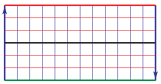
\includegraphics{mobiusC.pdf}
\end{center}
\end{efig}
}
Lay it flat and then introduce a half twist so that the arrow on the right hand
end points upwards, rather than downwards. Then glue the two ends of the strip
together, with the two arrows coinciding. That's the M\"obius strip.
\begin{efig}
\begin{center}
     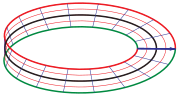
\includegraphics{mobiusB.pdf}
\end{center}
\end{efig}

Let's parametrize it. Think of the strip of paper that we used to construct 
it as consisting of a backbone (the horizontal black line in the figure below) 
with a bunch of ribs (like the thick blue line in the figure) emanating from it.
\vadjust{
\begin{efig}
\begin{center}
     \includegraphics{mobiusD.pdf}
\end{center}
\end{efig}
}
When we glue the two  ends of the strip together, the black line forms
a circle. If the strip has length $\ell$, the circle will have circumference $\ell$ and hence radius $\frac{\ell}{2\pi}$. We'll parametrize it as 
the circle
\begin{align*}
\frac{\ell}{2\pi}\hr(\theta)
\qquad\text{where } \hr(\theta) = \cos(\theta)\,\hi + \sin(\theta)\,\hj 
\end{align*}
This circle is in the $xy$-plane. It is the black circle in the 
figure below. (The figure only shows the part of the circle 
in the first octant, i.e. with $x,y,z\ge 0$.)
\vadjust{
\begin{efig}
\begin{center}
     \includegraphics{mobiusE.pdf}
\end{center}
\end{efig}
}
Now we'll add in the blue ribs. We'll put the blue rib, that is attached to 
the backbone at $\frac{\ell}{2\pi}\hr(\theta)$, in the plane
that contains the vectors $\hr(\theta)$ and $\hk$. 
%That way the blue rib is perpendicular to the red backbone.
A side view of the plane that contains the vectors $\hr(\theta)$ and $\hk$
is sketched in the figure below. 
\vadjust{
\begin{efig}
\begin{center}
     \includegraphics{mobiusF.pdf}
\end{center}
\end{efig}
}
To put the half twist into the strip of paper, we want the 
blue rib to rotate about the backbone by $180^\circ$, i.e. $\pi$ radians, 
as $\theta$ runs from $0$ to $2\pi$. That 
will be the case if we pick the angle $\varphi$ in the figure to be
$\nicefrac{\theta}{2}$. The vector that is running along the blue rib
in the figure is
\begin{equation*}
\vu(v,\theta,\varphi)=v\cos(\varphi)\,\hr(\theta) + v\sin(\varphi)\,\hk
%=v\cos(\nicefrac{\theta}{2})\,\hr(\theta) + v\sin(\nicefrac{\theta}{2})\,\hk
\end{equation*}  
where the length, $v$, of the vector is a parameter.
If the width of our original strip of paper is $w$, then as the parameter
$v$ runs from $-\nicefrac{w}{2}$ to $+\nicefrac{w}{2}$, the tip of the
vector $\vu(v,\theta,\varphi)$ runs over the entire blue rib. 
So, choosing $\varphi=\nicefrac{\theta}{2}$, our parametrization 
of the M\"obius strip is
\begin{align*}
\vr(\theta,v) 
 &= \frac{\ell}{2\pi}\hr(\theta) 
             + \vu(v,\theta,\nicefrac{\theta}{2}) \\
 &= \frac{\ell}{2\pi}\hr(\theta) 
     + v\cos\big(\nicefrac{\theta}{2}\big) \hr(\theta)
      + v\sin\big(\nicefrac{\theta}{2}\big) \hk
\qquad 0\le\theta<2\pi,\ -\frac{w}{2}\le v\le \frac{w}{2}
\end{align*}
where $\hr(\theta) = \cos(\theta)\,\hi + \sin(\theta)\,\hj$. 

Now that we have parametrized the M\"obius strip, let's return to
the question of orientability. Recall, from Definition \ref{def:oriented},
that, if the M\"obius strip were orientable, there would exist a continuous
function $\hN$ which assigns to each point $\vr$ of the strip a unit 
normal vector $\hN(\vr)$ at $\vr$. First, we'll find the normal vectors
to the surface using \eqref{eq:SUdSparam}. The partial derivatives
\begin{align*}
\frac{\partial\vr}{\partial\theta}(\theta,v)
&=\frac{\ell}{2\pi}\hr'(\theta) 
     + v\cos\big(\nicefrac{\theta}{2}\big) \hr'(\theta)
     - \frac{v}{2}\sin\big(\nicefrac{\theta}{2}\big) \hr(\theta)
     + \frac{v}{2}\cos\big(\nicefrac{\theta}{2}\big) \hk
\\
\frac{\partial\vr}{\partial v}(\theta,v)
&=\cos\big(\nicefrac{\theta}{2}\big) \hr(\theta)
      + \sin\big(\nicefrac{\theta}{2}\big) \hk
\end{align*}
are relatively messy, so let's just consider the case $v=0$ 
(i.e. find the normal vectors on the backbone).
Then
\begin{align*}
\frac{\partial\vr}{\partial\theta}(\theta,0)
&=\frac{\ell}{2\pi}\hr'(\theta) 
\\
\frac{\partial\vr}{\partial v}(\theta,0)
&=\cos\big(\nicefrac{\theta}{2}\big) \hr(\theta)
      + \sin\big(\nicefrac{\theta}{2}\big) \hk
\end{align*}
Since
\begin{align*}
\hr'(\theta)\times \hr(\theta)
&=\big(-\sin(\theta)\,\hi + \cos(\theta)\,\hj\big)\times
   \big(\cos(\theta)\,\hi + \sin(\theta)\,\hj\big)
=-\hk
\\
\hr'(\theta)\times \hk
&=\big(-\sin(\theta)\,\hi + \cos(\theta)\,\hj\big)\times \hk
=\hr(\theta)
\end{align*}
we have
\begin{align*}
\frac{\partial\vr}{\partial\theta}(\theta,0) \times 
\frac{\partial\vr}{\partial v}(\theta,0)
=-\frac{\ell}{2\pi}\Big(\cos\big(\nicefrac{\theta}{2}\big)\,\hk
                       -\sin\big(\nicefrac{\theta}{2}\big)\,\hr(\theta) \Big)
\end{align*}
As $\hk$ and $\hr(\theta)$ are mutually perpendicular unit vectors,
$\cos\big(\nicefrac{\theta}{2}\big)\,\hk
                       -\sin\big(\nicefrac{\theta}{2}\big)\,\hr(\theta)$ 
has length one, and the two unit normal vectors to the M\"obius strip
at $\vr(\theta,0)$ are
\begin{equation*}
\pm \Big(\cos\big(\nicefrac{\theta}{2}\big)\,\hk
                       -\sin\big(\nicefrac{\theta}{2}\big)\,\hr(\theta) \Big)
\end{equation*}
So, for each $\theta$, $\hN\big(\vr(\theta,0)\big)$ must be either 
\begin{equation*}
\cos\big(\nicefrac{\theta}{2}\big)\,\hk
                       -\sin\big(\nicefrac{\theta}{2}\big)\,\hr(\theta)
\qquad\text{or}\qquad 
-\big(\cos\big(\nicefrac{\theta}{2}\big)\,\hk
                       -\sin\big(\nicefrac{\theta}{2}\big)\,\hr(\theta) \big)
\end{equation*}
Imagine walking along the M\"obius strip.
The normal vector $\hN\big(\vr(\theta,v)\big)$ is our body when we are 
at $\vr(\theta,v)$ --- our feet are at the tail of the vector 
$\hN\big(\vr(\theta,v)\big)$ and our head is at the arrow of 
$\hN\big(\vr(\theta,v)\big)$. We start walking at 
$\vr(0,0)=\frac{\ell}{2\pi}\hi$. Our body,
$\hN\big(\frac{\ell}{2\pi}\hi\big)=\hN\big(\vr(0,0)\big)$ has to be one of 
$\pm \big(\cos(0)\,\hk-\sin(0)\,\hr(0) \big)=\pm\hk$. 
Let's suppose that $\hN\big(\vr(0,0)\big)=+\hk$. (We start upright.)
Now we start walking along the backbone of the M\"obius strip, 
increasing $\theta$. Because $\hN\big(\vr(\theta,0)\big)$ has to be continuous, 
$\hN\big(\vr(\theta,0)\big)$ has to be 
$+\big(\cos\big(\nicefrac{\theta}{2}\big)\,\hk
                       -\sin\big(\nicefrac{\theta}{2}\big)\,\hr(\theta) \big)$.
We keep increasing $\theta$. By continuity, $\hN\big(\vr(\theta,0)\big)$ has to be 
$+\big(\cos\big(\nicefrac{\theta}{2}\big)\,\hk
                       -\sin\big(\nicefrac{\theta}{2}\big)\,\hr(\theta) \big)$
for bigger and bigger $\theta$. Eventually we get to $\theta=2\pi$, i.e. to
\begin{equation*}
\vr(2\pi,0)= \frac{\ell}{2\pi}\hr(2\pi) =  \frac{\ell}{2\pi}\hi
=\frac{\ell}{2\pi}\hr(0)=\vr(0,0)
\end{equation*}
We are back to our starting point. Continuity has forced
\begin{equation*}
\hN\big(\vr(2\pi,0)\big)
=\hN\big(\vr(\theta,0)\big)\Big|_{\theta=2\pi}
=+\big(\cos\big(\nicefrac{\theta}{2}\big)\,\hk
                       -\sin\big(\nicefrac{\theta}{2}\big)\,\hr(\theta) \big)
\Big|_{\theta=2\pi}
=-\hk
\end{equation*}
So we have arrived back upside down.
That's a problem --- $\hN\big(\vr(2\pi,0)\big)
=\hN\big(\frac{\ell}{2\pi}\hi\big)$
and we have already defined $\hN\big(\frac{\ell}{2\pi}\hi\big)=+\hk$, not $-\hk$. So the M\"obius strip is not orientable. The interested reader
should look up M. C. Escher's M\"obius Strip II (Red Ants).

\end{eg}









